% !TeX root = ../main.tex

\chapter{相关技术基础}
本文工作开展在基于深度学习的神经辐射场之上,通过结合可微渲染实现了数字资产解耦管线,
致力于无缝对接传统渲染管线并解决其中的耦合问题。本章将介绍本文研究所必要的深度学习基础、
可微渲染理论基础、传统渲染管线介绍以及神经辐射场理论基础。

\section{深度学习基础}
【这里应该加点引言之类的】
\subsection{基于坐标的多层感知机}
多层感知机(Multilayer Perceptron,MLP)作为深度学习的基础模型,由感知机推广而来,
本质是一种前馈神经网络。MLP由多个神经元层组成,每个神经元的结构如图~\ref{fig:neuron}所示,其接收多个输入值,
并按照自身权重进行加权求和,接着,使用激活函数对其进行非线性变换,并将变换后的值传递给下一层神经元。

\begin{figure}[htb]
  \centering
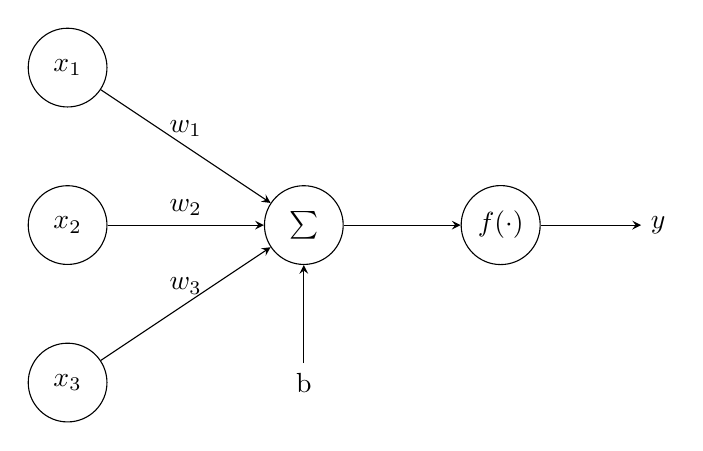
\begin{tikzpicture}[->,>=stealth, node distance=1.5cm, auto]
  % 定义输入节点
  \node[circle, draw, minimum size=1cm] (x1) at (0, 2) {$x_1$};
  \node[circle, draw, minimum size=1cm] (x2) at (0, 0) {$x_2$};
  \node[circle, draw, minimum size=1cm] (x3) at (0, -2) {$x_3$};

  % 定义偏置节点
  \node (bias) at (3, -2) {$\mathrm{b}$};

  % 定义神经元节点,内部写上激活函数(如 f(·))
  \node[circle, draw, minimum size=1cm] (sum) at (3, 0) {$\sum$};

  % 从输入节点到神经元的连线,并标注权重
  \draw (x1) -- node[midway, above] {$w_1$} (sum);
  \draw (x2) -- node[midway, above] {$w_2$} (sum);
  \draw (x3) -- node[midway, above] {$w_3$} (sum);
  % 从偏置节点到神经元的连线,标注偏置项
  \draw (bias) -- node[midway, below] {}(sum);

  % 定义神经元节点,内部写上激活函数(如 f(·))
  \node[circle, draw, minimum size=1cm] (activate) at (5.5, 0) {$f(\cdot)$};

  \node (y) at (7.5, 0) {$y$};

  \draw (sum) -- node[midway, below] {}(activate);
  \draw (activate) -- node[midway, below] {}(y);
\end{tikzpicture}
\caption{神经元的结构示意图}
\label{fig:neuron}
\end{figure}

多层感知机通过神经元从输入数据中学习到合适的参数权重和偏置项,利用激活函数将线性关系转化为非线性信号,
使得网络能够准确地完成各种分类或回归预测等方面的任务。这些信号从输入层通过一系列的隐藏层最终输出到输出层,
各层之间是完全连接的,具体如图~\ref{fig:mlp}所示:

\begin{figure}[htb]
  \centering
  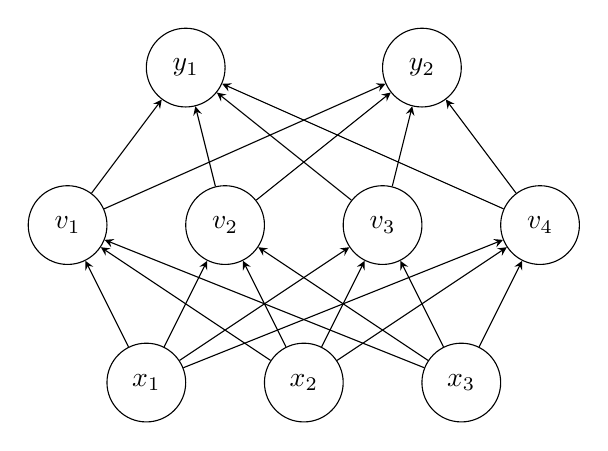
\begin{tikzpicture}[>=stealth, auto]

    % 定义公共变量
    \def\xspacing{2}      % 输入层和隐藏层的水平间距
    \def\layersep{2}       % 垂直层间距
    
    % 定义输出层特有的水平间距(可以调大该值)
    \def\outputxspacing{3} % 输出层水平间距
  
    % 输入层:3个节点
    \foreach \i in {1,...,3} {
      \pgfmathsetmacro{\xpos}{(\i-2)*\xspacing};
      \node[circle, draw, minimum size=1cm] (x\i) at (\xpos, 0) {$x_{\i}$};
    }
  
    % 隐藏层:4个节点
    \foreach \i in {1,...,4} {
      \pgfmathsetmacro{\xpos}{(\i-2.5)*\xspacing};
      \node[circle, draw, minimum size=1cm] (v\i) at (\xpos, \layersep) {$v_{\i}$};
    }
  
    % 输出层:2个节点,使用新的水平间距
    \foreach \i in {1,...,2} {
      \pgfmathsetmacro{\xpos}{(\i-1.5)*\outputxspacing};
      \node[circle, draw, minimum size=1cm] (y\i) at (\xpos, 2*\layersep) {$y_{\i}$};
    }
  
    % 连接输入层到隐藏层(全连接)
    \foreach \i in {1,...,3} {
      \foreach \j in {1,...,4} {
        \draw[->] (x\i) -- (v\j);
      }
    }
    
    % 连接隐藏层到输出层(全连接)
    \foreach \i in {1,...,4} {
      \foreach \j in {1,...,2} {
        \draw[->] (v\i) -- (y\j);
      }
    }
  
  \end{tikzpicture}
\caption{多层感知机的结构示意图}
\label{fig:mlp}
\end{figure}

根据通用近似定理\cite{Hornik_1989},只要给予网络足够多的神经元,MLP即可以任意精度逼近紧致集上的连续函数,
这一理论奠定了MLP作为函数逼近器的数学基础。然而,传统MLP多用于处理向量化特征(如图像分类中的扁平化像素),
其输入空间通常缺乏明确的几何语义。基于坐标的多层感知机(Coordinate-based MLPs)则突破了这一局限,
通过将空间坐标直接作为网络输入,并引入傅里叶坐标编码(Fourier Positional Encoding)
进行频域编码\cite{tancik2020fourier},
实现了对连续场函数的隐式建模,从而开创了三维几何与信号表示的新范式。

具体而言,直接使用原始坐标作为输入会导致 MLP 呈现明显的频谱偏差问题\cite{pmlr-v97-rahaman19a}。由于网络倾向于优先学习低频信号,
导致网络难以捕捉三维几何中的高频细节(如表面纹理、尖锐边缘等)。为此,研究者提出利用傅里叶坐标编码,
将 $d$ 维坐标 $\mathbf{x}\in\mathbb{R}^d$ 通过傅里叶基函数投影至高维空间。
傅里叶坐标编码可以由公式\eqref{eq:fourier_encoding}表示:
\begin{equation}
\gamma(\mathbf{x})=\left[\sin\left(2^0\pi \mathbf{x}\right),\cos\left(2^\pi \mathbf{x}\right),\ldots,\sin\left(2^{K-1}\pi \mathbf{x}\right),\cos\left(2^{K-1}\pi \mathbf{x}\right)\right]
\label{eq:fourier_encoding}
\end{equation}
其中 $K$ 为预设的频率层级,通过指数增长的频率项构造多尺度频带。
这种傅里叶坐标编码(Fourier Positional Encoding)使MLP能够显式访问不同频段的几何特征,
有效解决了频谱偏差问题。在神经辐射场(NeRF)等典型应用中,该技术被证明是实现高质量三维重建的关键因素。

\subsection{激活函数}

通过上文的介绍我们知道,在多层神经网络中,隐藏层仅能进行线性变换,因此仅由隐藏层组成的线性模型只
能拟合输入和输出之间的线性关系,无法处理非线性问题。为了增强模型的非线性表示能力,可以使用激活函数来加入非线性因素。
由于不同类型的激活函数对提高网络的非线性表示能力不同,所以针对不同的任务需要选择适合的激活函数。
多层感知机使用的常见激活函数有Sigmoid函数,ELU(Exponential Linear Unit)以及ReLU(Rectified Linear Unit)。

\fourthtitle{1}Sigmoid激活函数

Sigmoid激活函数是一种平滑的奇函数,该函数与其导数的计算方式如公式\ref{eq:sigmoid}所示:
\begin{equation}
  \begin{aligned}
  \text{Sigmoid}(x) &= \frac{1}{1+e^{-x}}, \\
  \text{Sigmoid}'(x) &= \text{Sigmoid}(x)\Bigl(1-\text{Sigmoid}(x)\Bigr).
  \end{aligned}
  \label{eq:sigmoid}
\end{equation}

Sigmoid函数的图像如图\ref{fig:sigmoid}所示,其输出范围在$(0,1)$之间,可以将任意实数映射到有限区间,
实现非线性变换。它曾广泛用于早期的神经网络,但当输入值较大或较小时,Sigmoid的导数会趋近于0,
有可能会导致深层网络出现梯度爆炸的问题。其次,由于Sigmoid的输出始终为正数,反向传播时,
所有层的权重更新方向相同。如果模型的最优权重包含正负值,这种更新方式降低训练过程的效率,影响收敛速度。

\begin{figure}[H]
  \centering
  \begin{subfigure}[t]{0.45\textwidth}
    \centering
    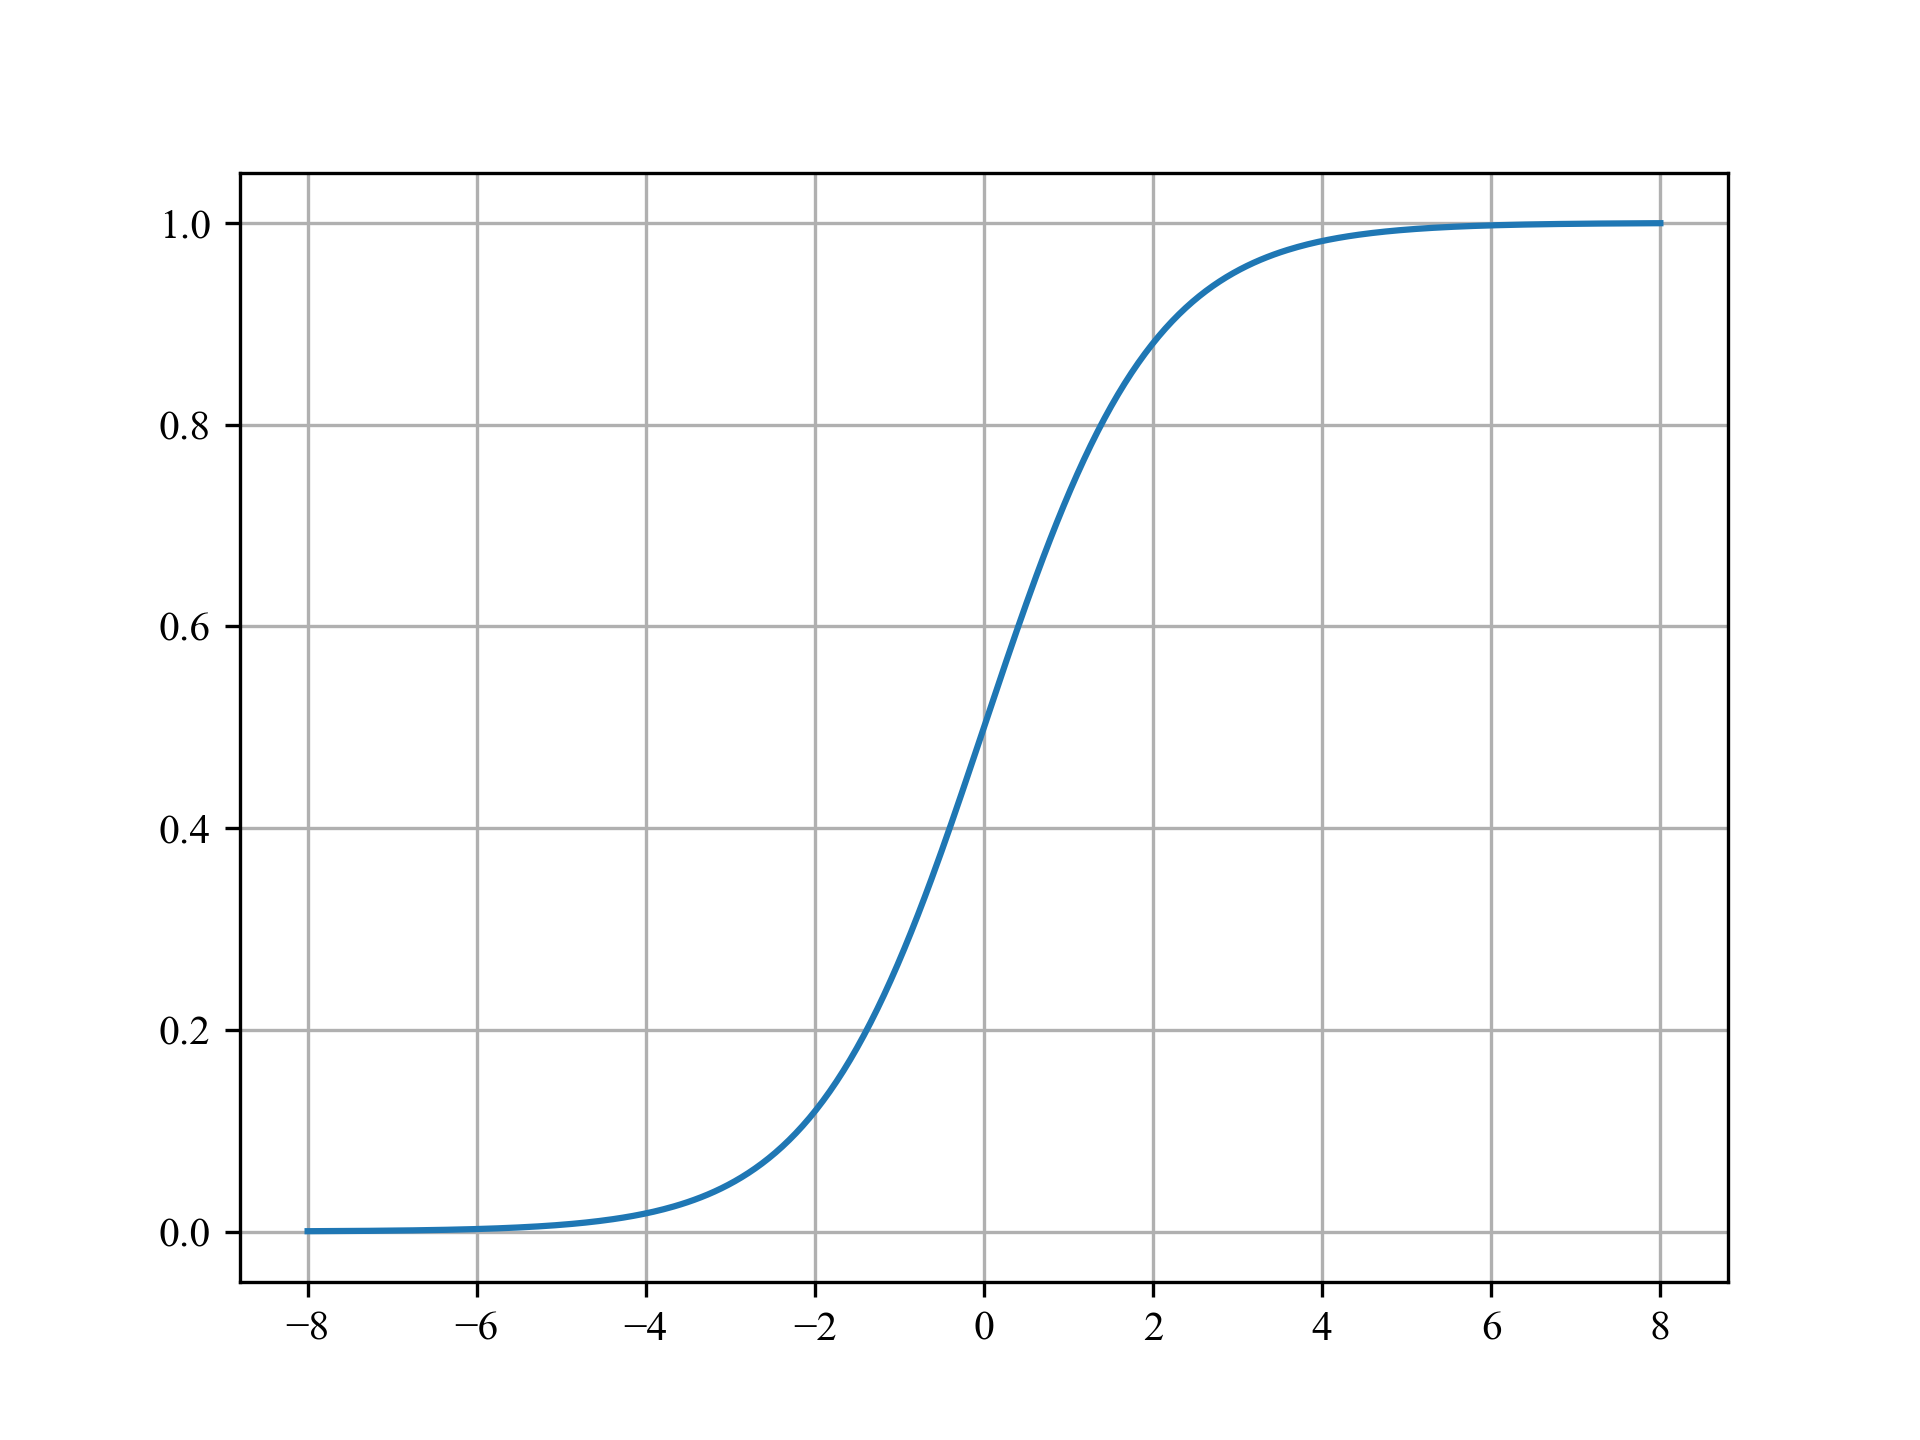
\includegraphics[width=\linewidth]{ch2/activation_function/sigmoid.png}
    \caption{Sigmoid函数图像}
  \end{subfigure}
  \begin{subfigure}[t]{0.45\textwidth}
    \centering
    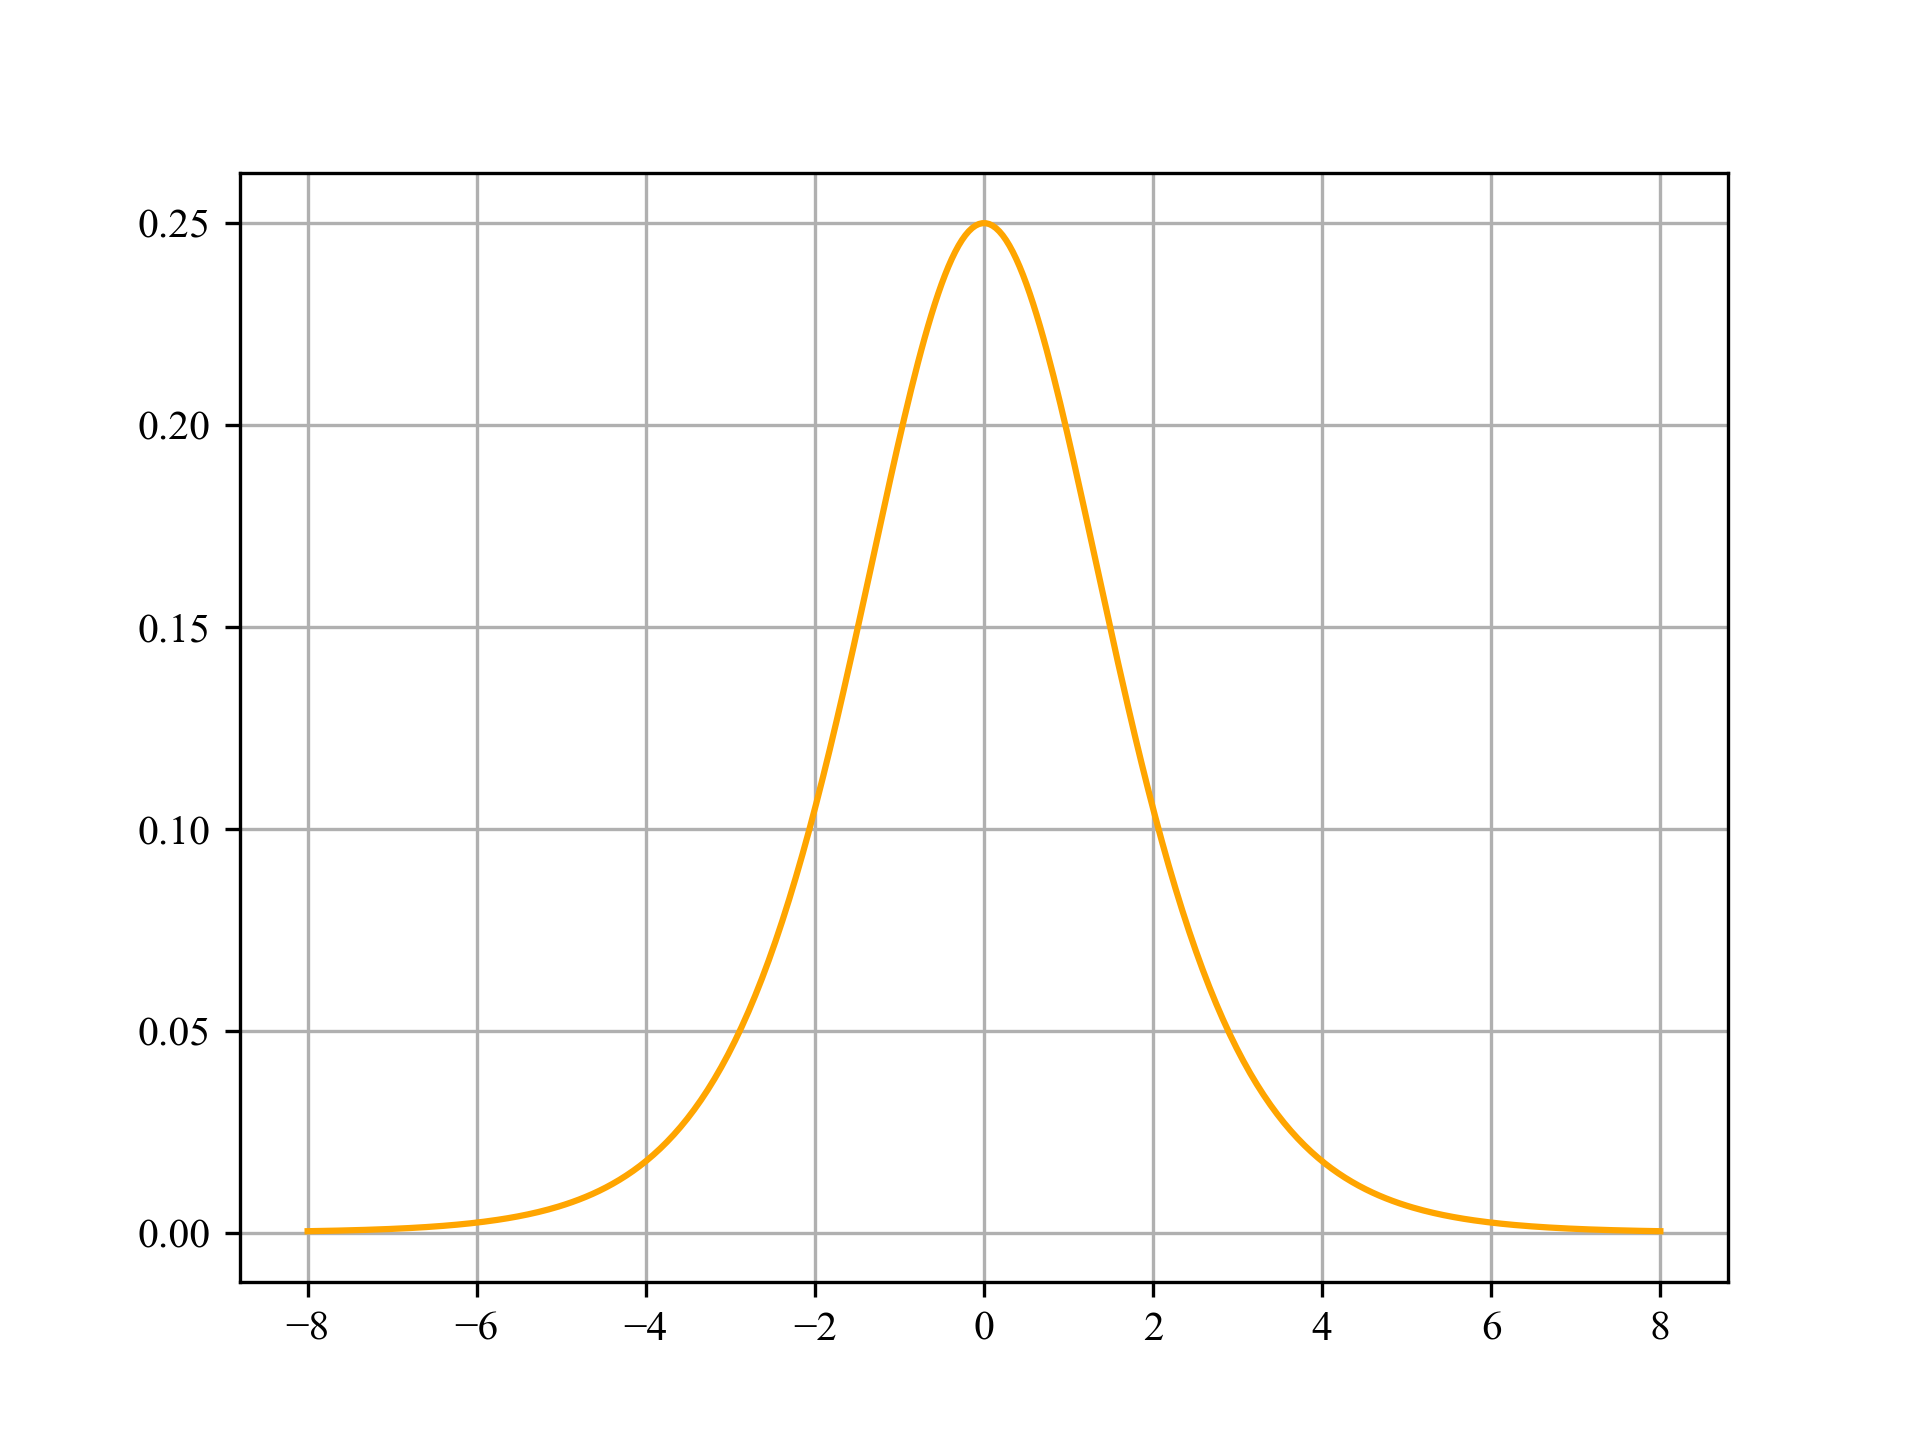
\includegraphics[width=\linewidth]{ch2/activation_function/dsigmoid.png}
    \caption{Sigmoid函数导数图像}
  \end{subfigure}
  \caption{Sigmoid激活函数及其导数图像}
  \label{fig:sigmoid}
\end{figure}

\fourthtitle{2} ReLU激活函数

ReLU激活函数由Nair等人\cite{Nair_Hinton_2010}提出,是一种分段函数,其基本表达式如公式\eqref{eq:relu}所示:
\begin{equation}
  \begin{aligned}
  \text{ReLU}(x) &= \begin{cases}
    0, & x < 0, \\
    x, & x > 0.
    \end{cases}
  \text{ReLU}'(x) &= \begin{cases}
  0, & x < 0, \\
  1, & x > 0.
  \end{cases}
  \end{aligned}
  \label{eq:relu}
\end{equation}

ReLU函数的图像如图\ref{fig:relu}所示,该函数近年来应用广泛。相较于Sigmoid函数,ReLU无需指数计算,因此计算效率更高。
同时,当输入大于0时,ReLU的导数始终为1,可以缓解梯度爆炸;当输入小于0时,ReLU输出为0,使得部分神经元不参与计算,
能够增强网络的稀疏性,但此时ReLU导数也为0,因此可能会导致某些神经元“死亡”,影响网络的训练和收敛。

\begin{figure}[H]
  \centering
  \begin{subfigure}[t]{0.45\textwidth}
    \centering
    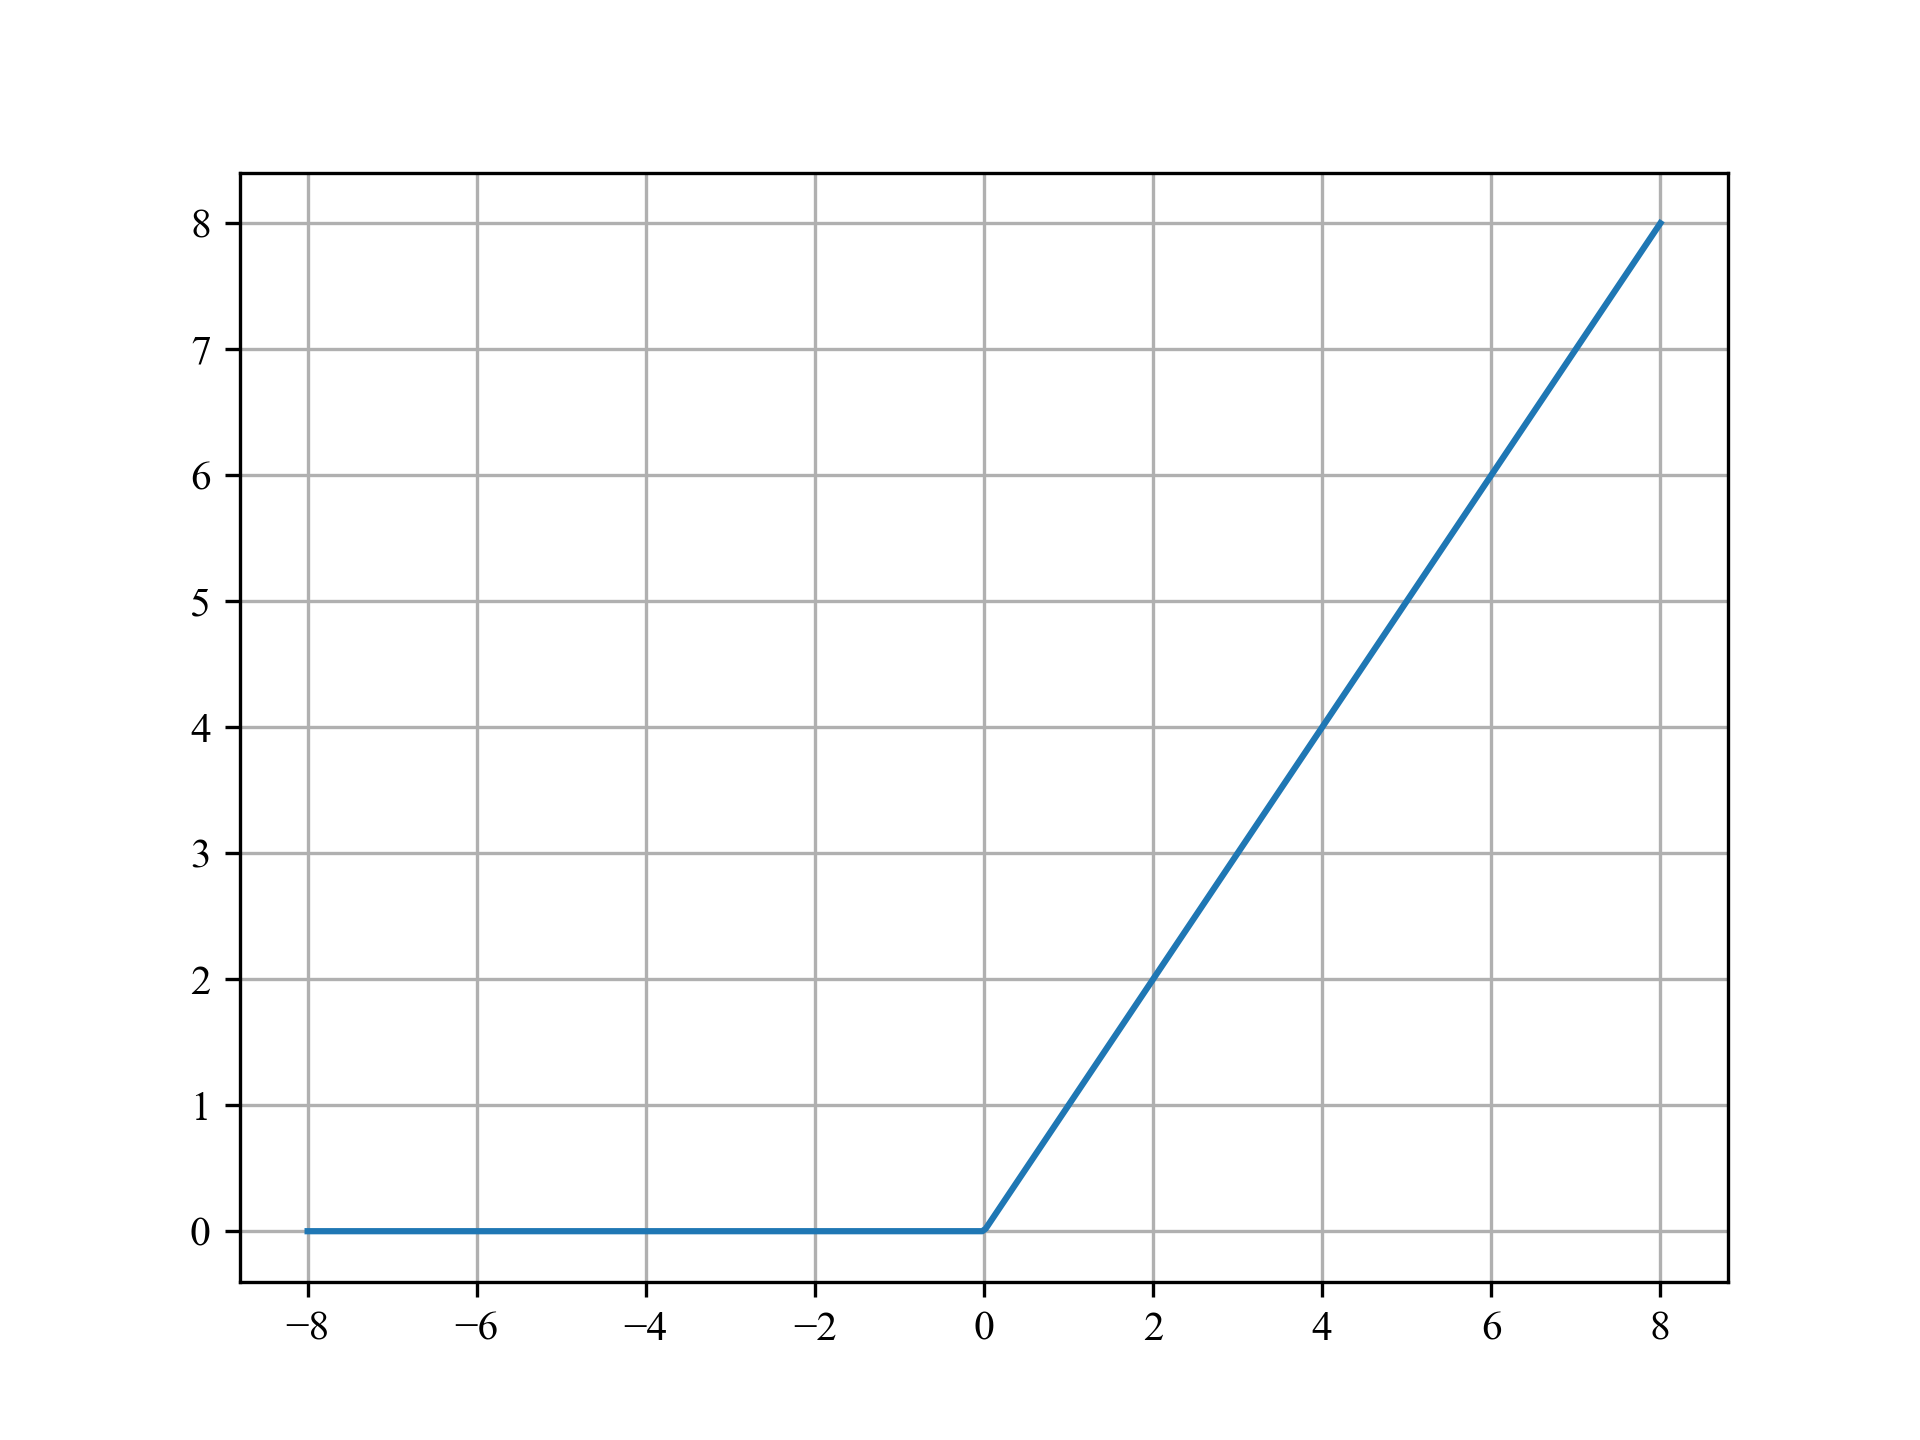
\includegraphics[width=\linewidth]{ch2/activation_function/relu.png}
    \caption{ReLU函数图像}
  \end{subfigure}
  \begin{subfigure}[t]{0.45\textwidth}
    \centering
    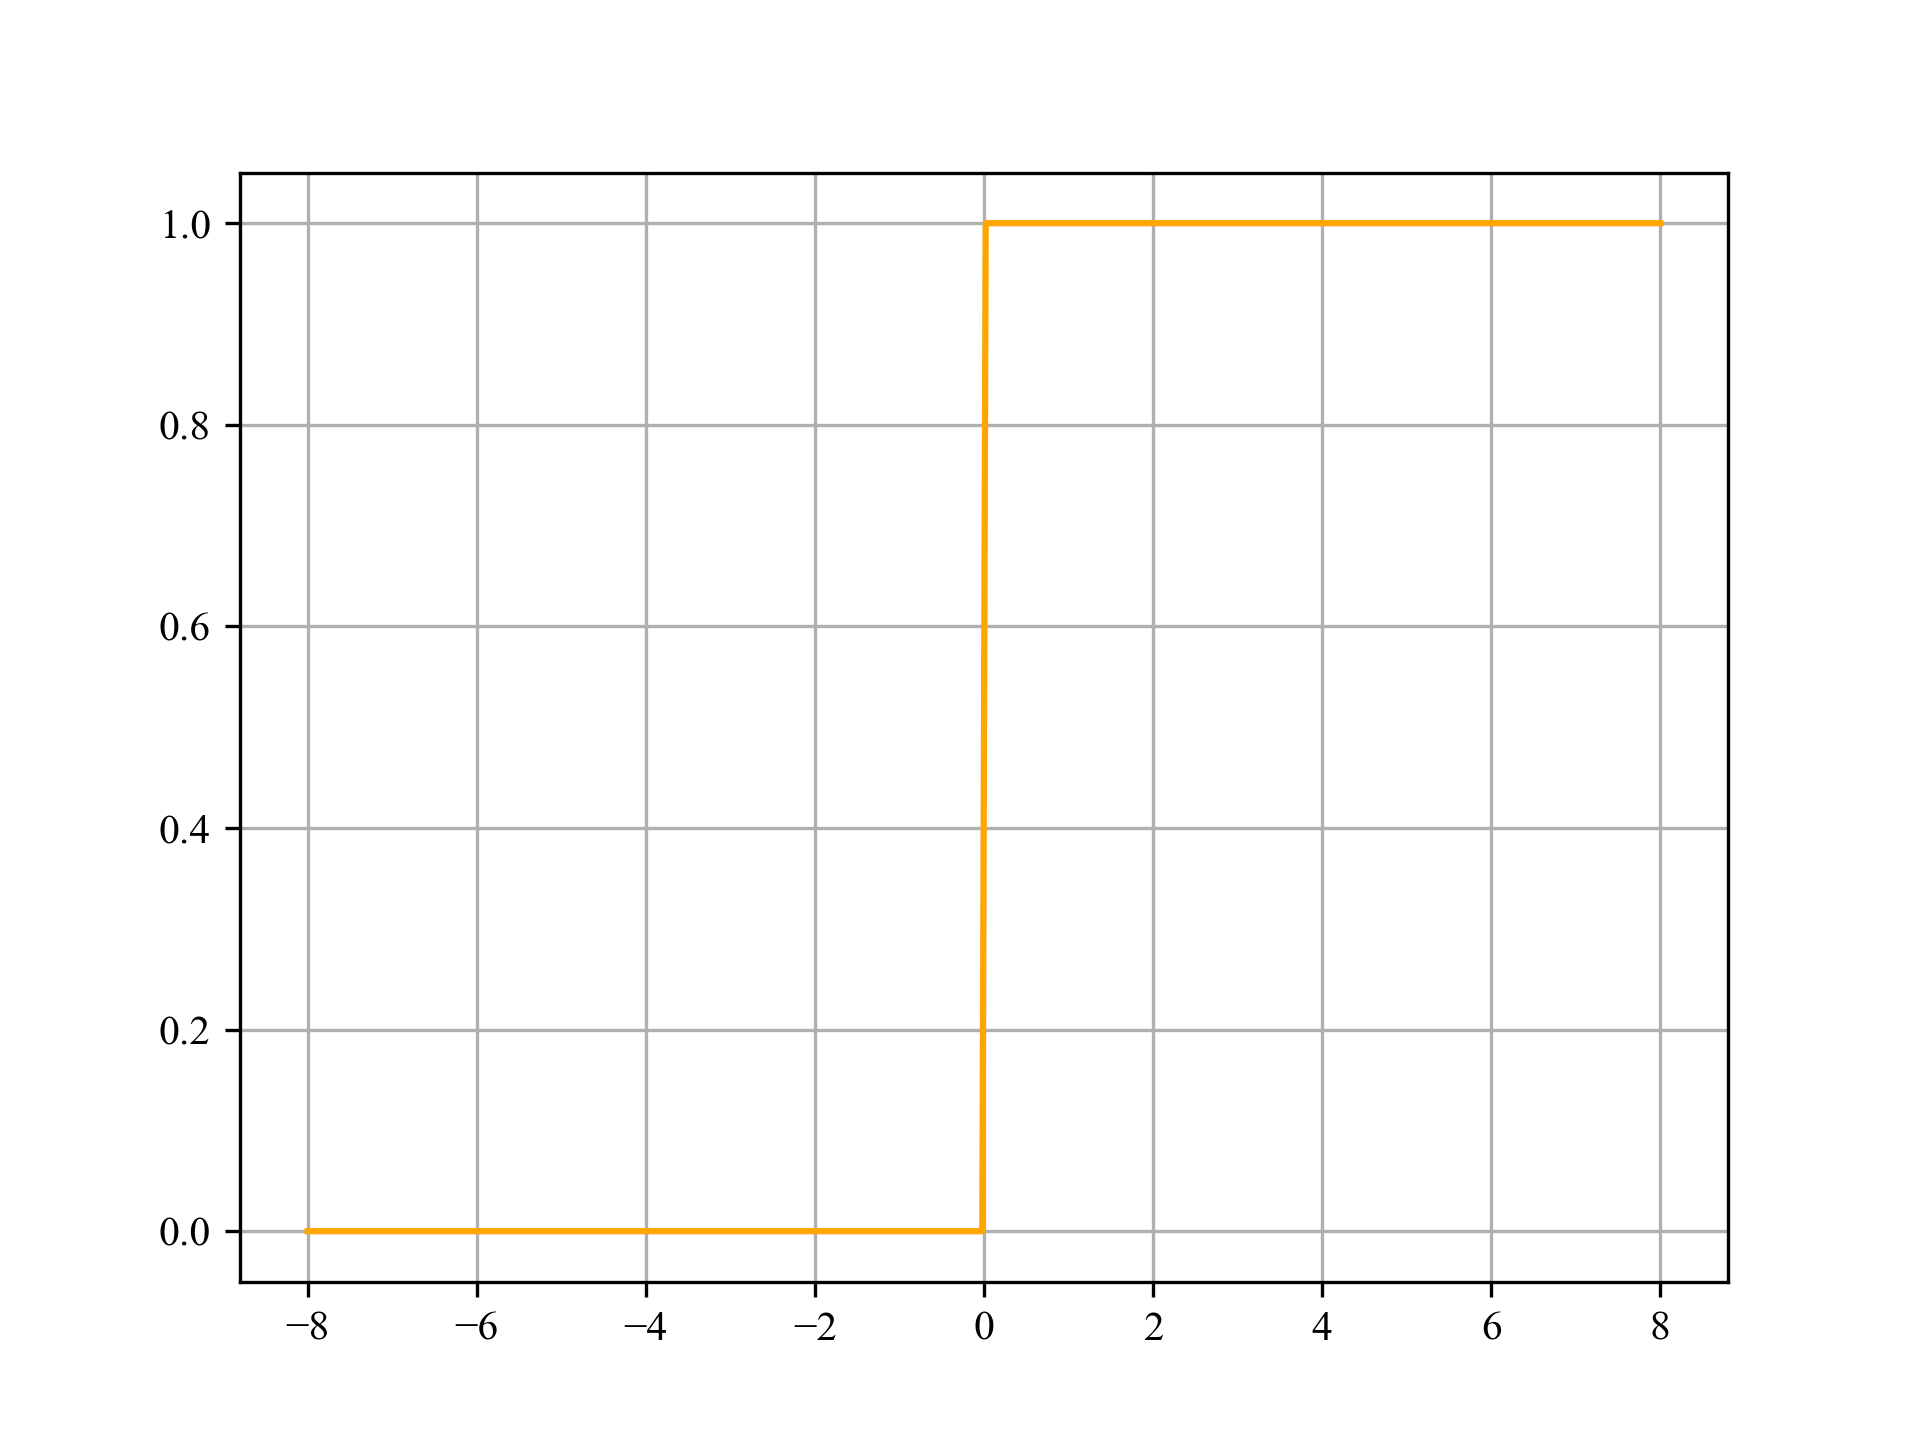
\includegraphics[width=\linewidth]{ch2/activation_function/drelu.png}
    \caption{ReLU函数导数图像}
  \end{subfigure}
  \caption{ReLU激活函数及其导数图像}
  \label{fig:relu}
\end{figure}

\fourthtitle{3} Elu激活函数

Elu激活函数由Clevert等人\cite{ClevertUH15}提出,旨在解决ReLU导致的神经元“死亡”问题,其计算方式如公式\eqref{eq:elu}所示:
\begin{equation}
  \begin{aligned}
  \text{ELU}(x) &= \begin{cases}
  x, & x \geq 0, \\
  \alpha \left(e^x - 1\right), & x < 0,
  \end{cases} \\
  \text{ELU}'(x) &= \begin{cases}
  1, & x \geq 0, \\
  \alpha e^x, & x < 0.
  \end{cases}
  \end{aligned}
  \label{eq:elu}
\end{equation}

Elu函数的图像如图\ref{fig:elu}所示。当输入大于0时,该函数行为类似于ReLU,其导数接近1,有助于保持梯度稳定,加快收敛速度;
当输入小于0时,Elu采用指数函数进行平滑衰减,使得激活值可以为负,有助于减少神经元“死亡”的情况。
同时,Elu函数引入了额外的超参数$\alpha$来控制负值部分的衰减程度。

\begin{figure}[H]
  \centering
  \begin{subfigure}[t]{0.45\textwidth}
    \centering
    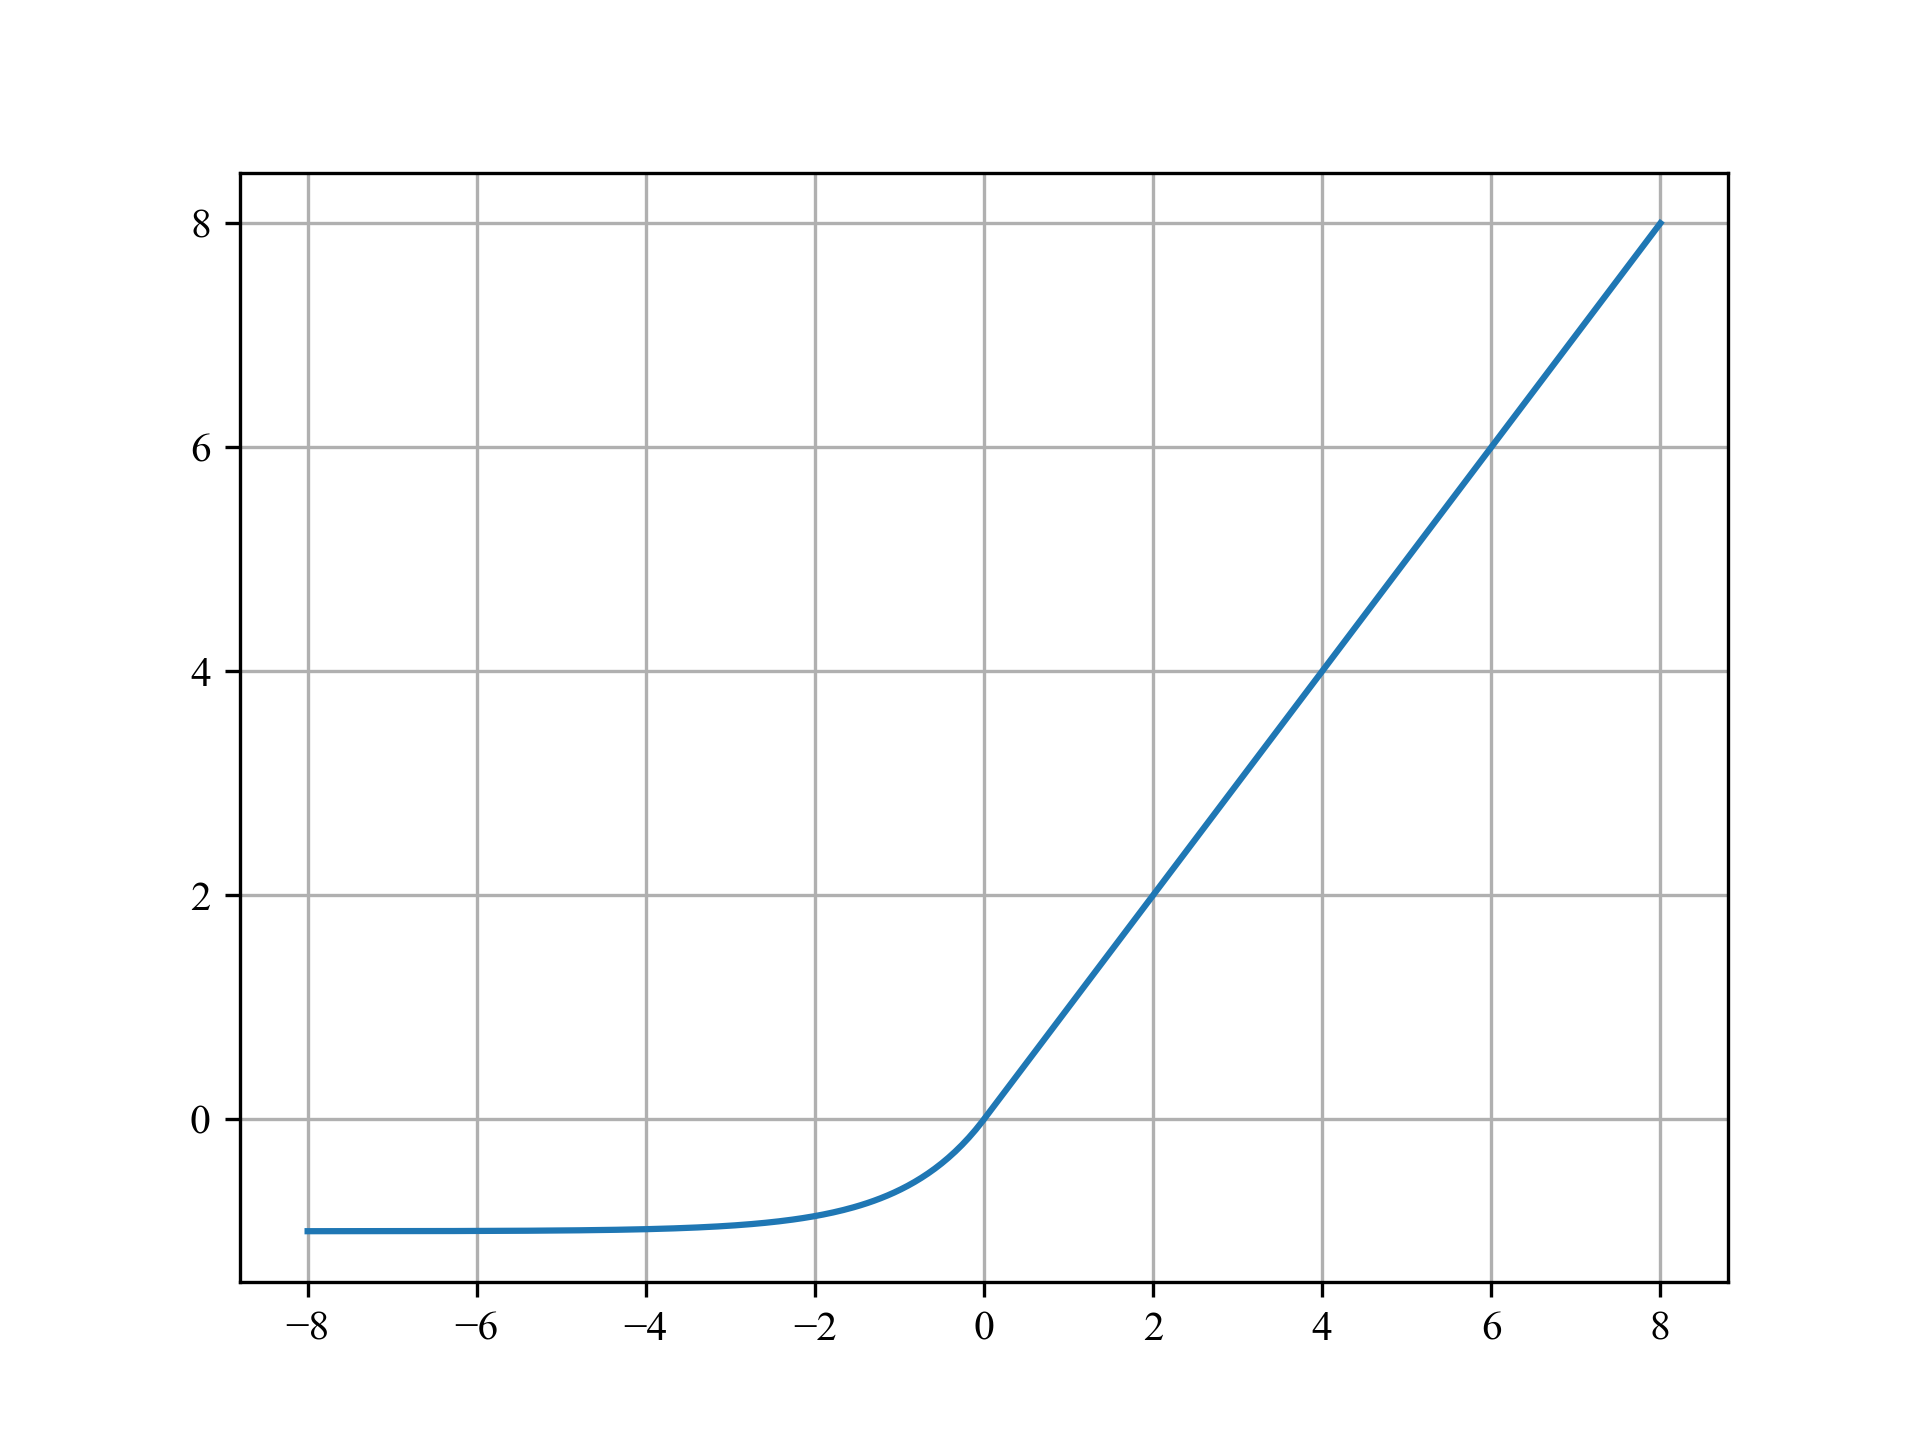
\includegraphics[width=\linewidth]{ch2/activation_function/elu.png}
    \caption{Elu函数图像}
  \end{subfigure}
  \begin{subfigure}[t]{0.45\textwidth}
    \centering
    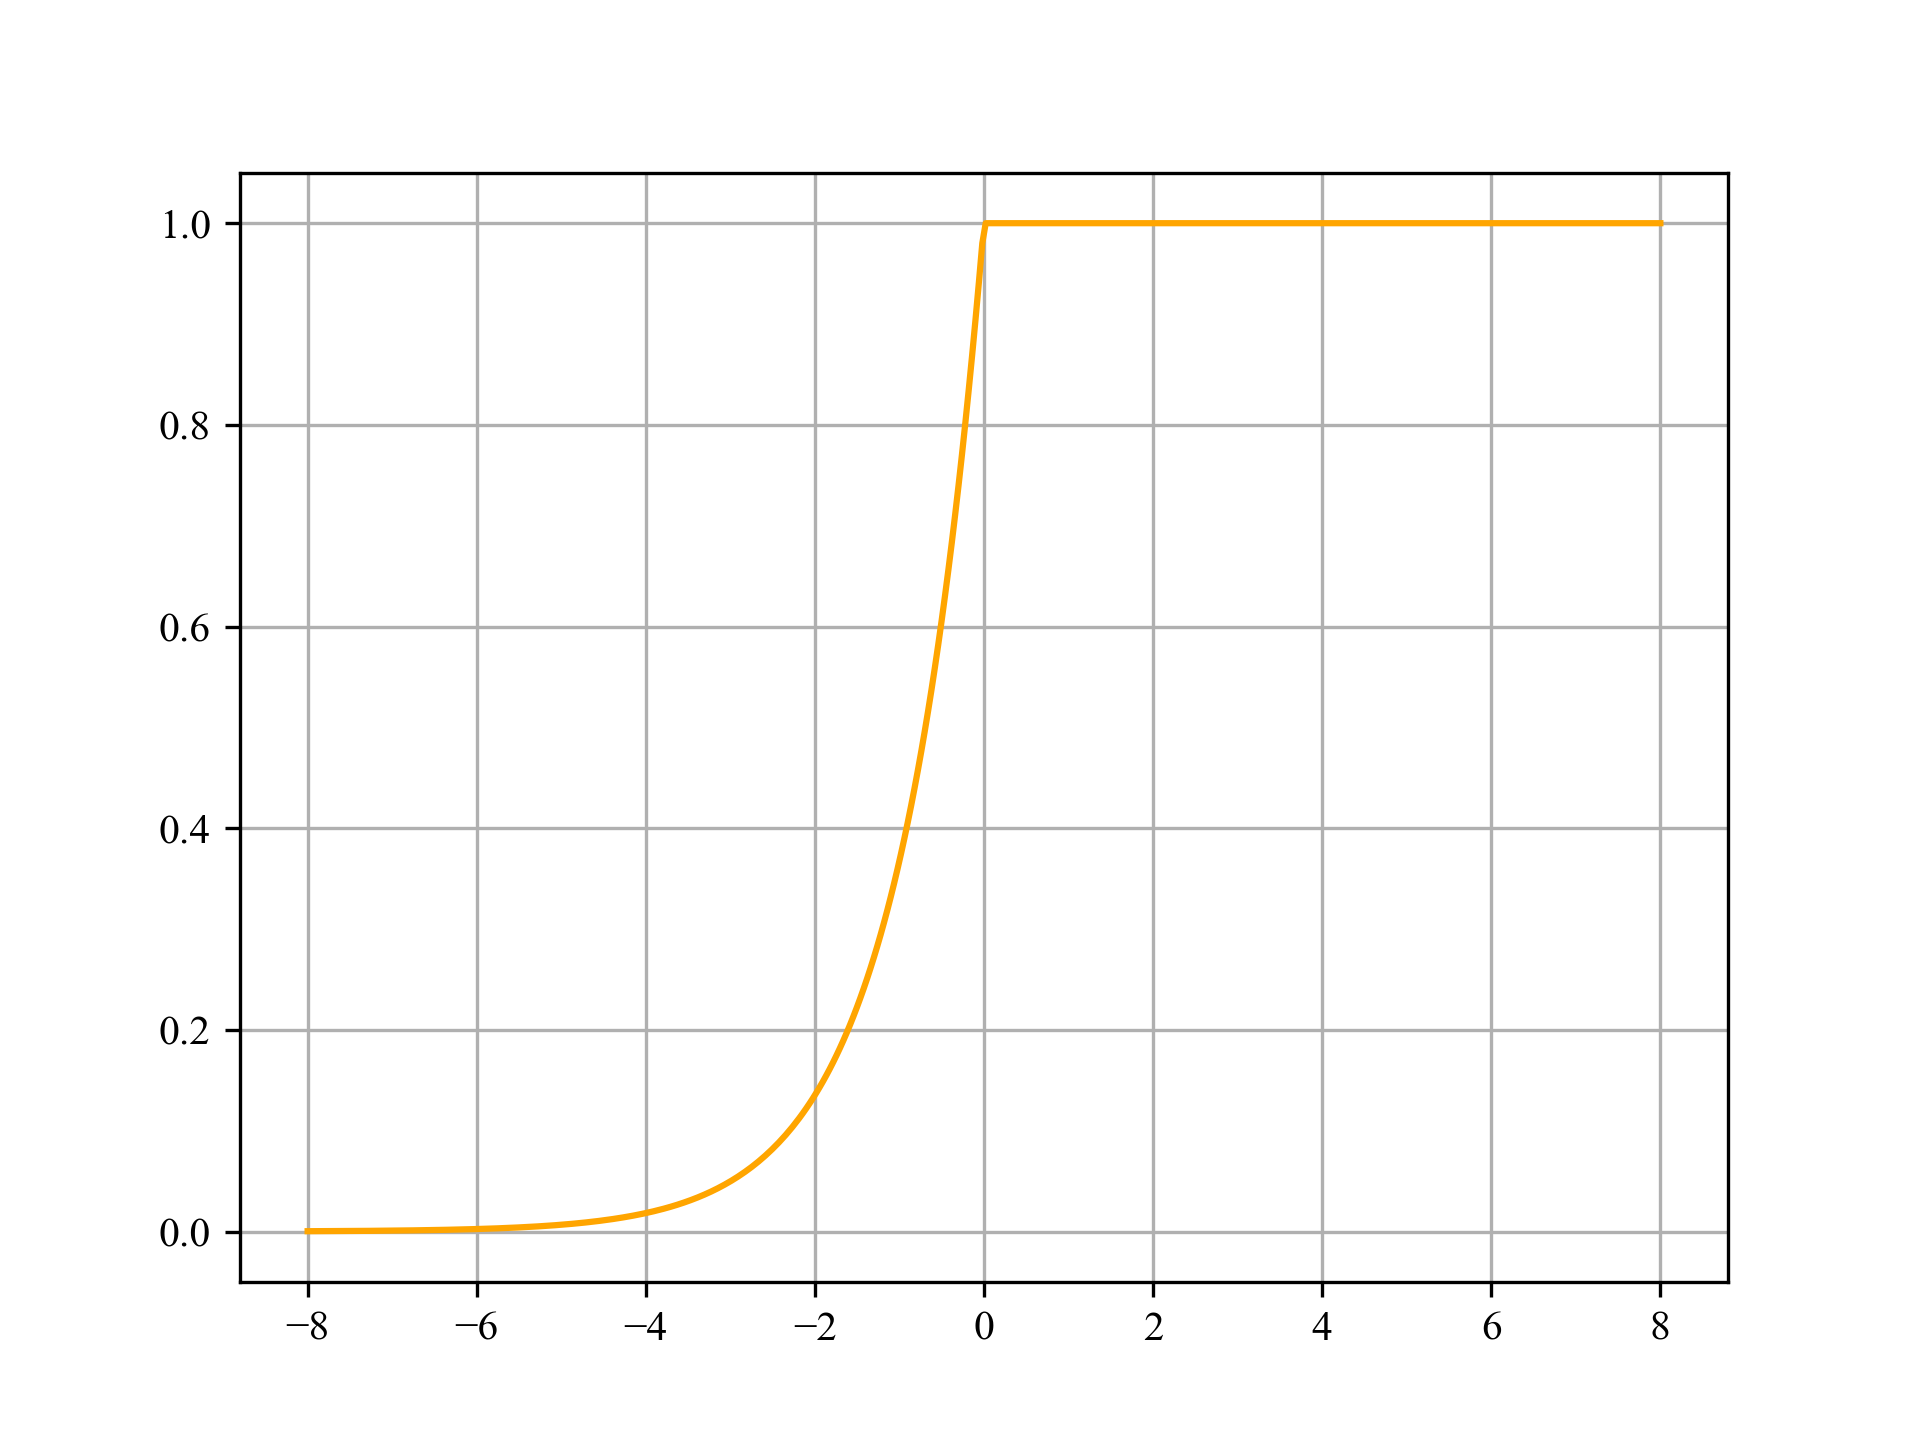
\includegraphics[width=\linewidth]{ch2/activation_function/delu.png}
    \caption{Elu函数导数图像}
  \end{subfigure}
  \caption{Elu激活函数及其导数图像}
  \label{fig:elu}
\end{figure}

\fourthtitle{4} SIREN激活函数

在基于坐标的多层感知机(MLP)中,传统激活函数往往导致网络学习过程中的频谱偏差问题。
为突破这一限制,Sitzmann 等人\cite{sitzmann2020implicit} 提出了SIREN(Sinusoidal Representation Networks),
其核心创新在于采用正弦函数作为激活函数。SIREN的激活函数定义如下:
\begin{equation}\label{eq:siren}
\phi_i(x_i)=\sin\Bigl(\omega_0\,W_i\,x_i+b_i\Bigr)
\end{equation}
其中,$\omega_0$ 是可学习的频率缩放因子,决定了正弦函数的振荡速率。与ReLU等常见激活函数不同,
正弦函数的周期性特性能够让网络更自然地表示高频信息。同时,正弦函数的导数始终非零,
使得梯度在网络层间传播时不易衰减,有助于学习复杂的细节信息。

此外,权重矩阵$W_i$与频率因子$\omega_0$共同影响输入信号的频域分布,
使网络能够自适应地平衡低频轮廓和高频细节的建模能力(如图\ref{fig:siren_compare} 所示)。

\begin{figure}[htb]
  \centering
  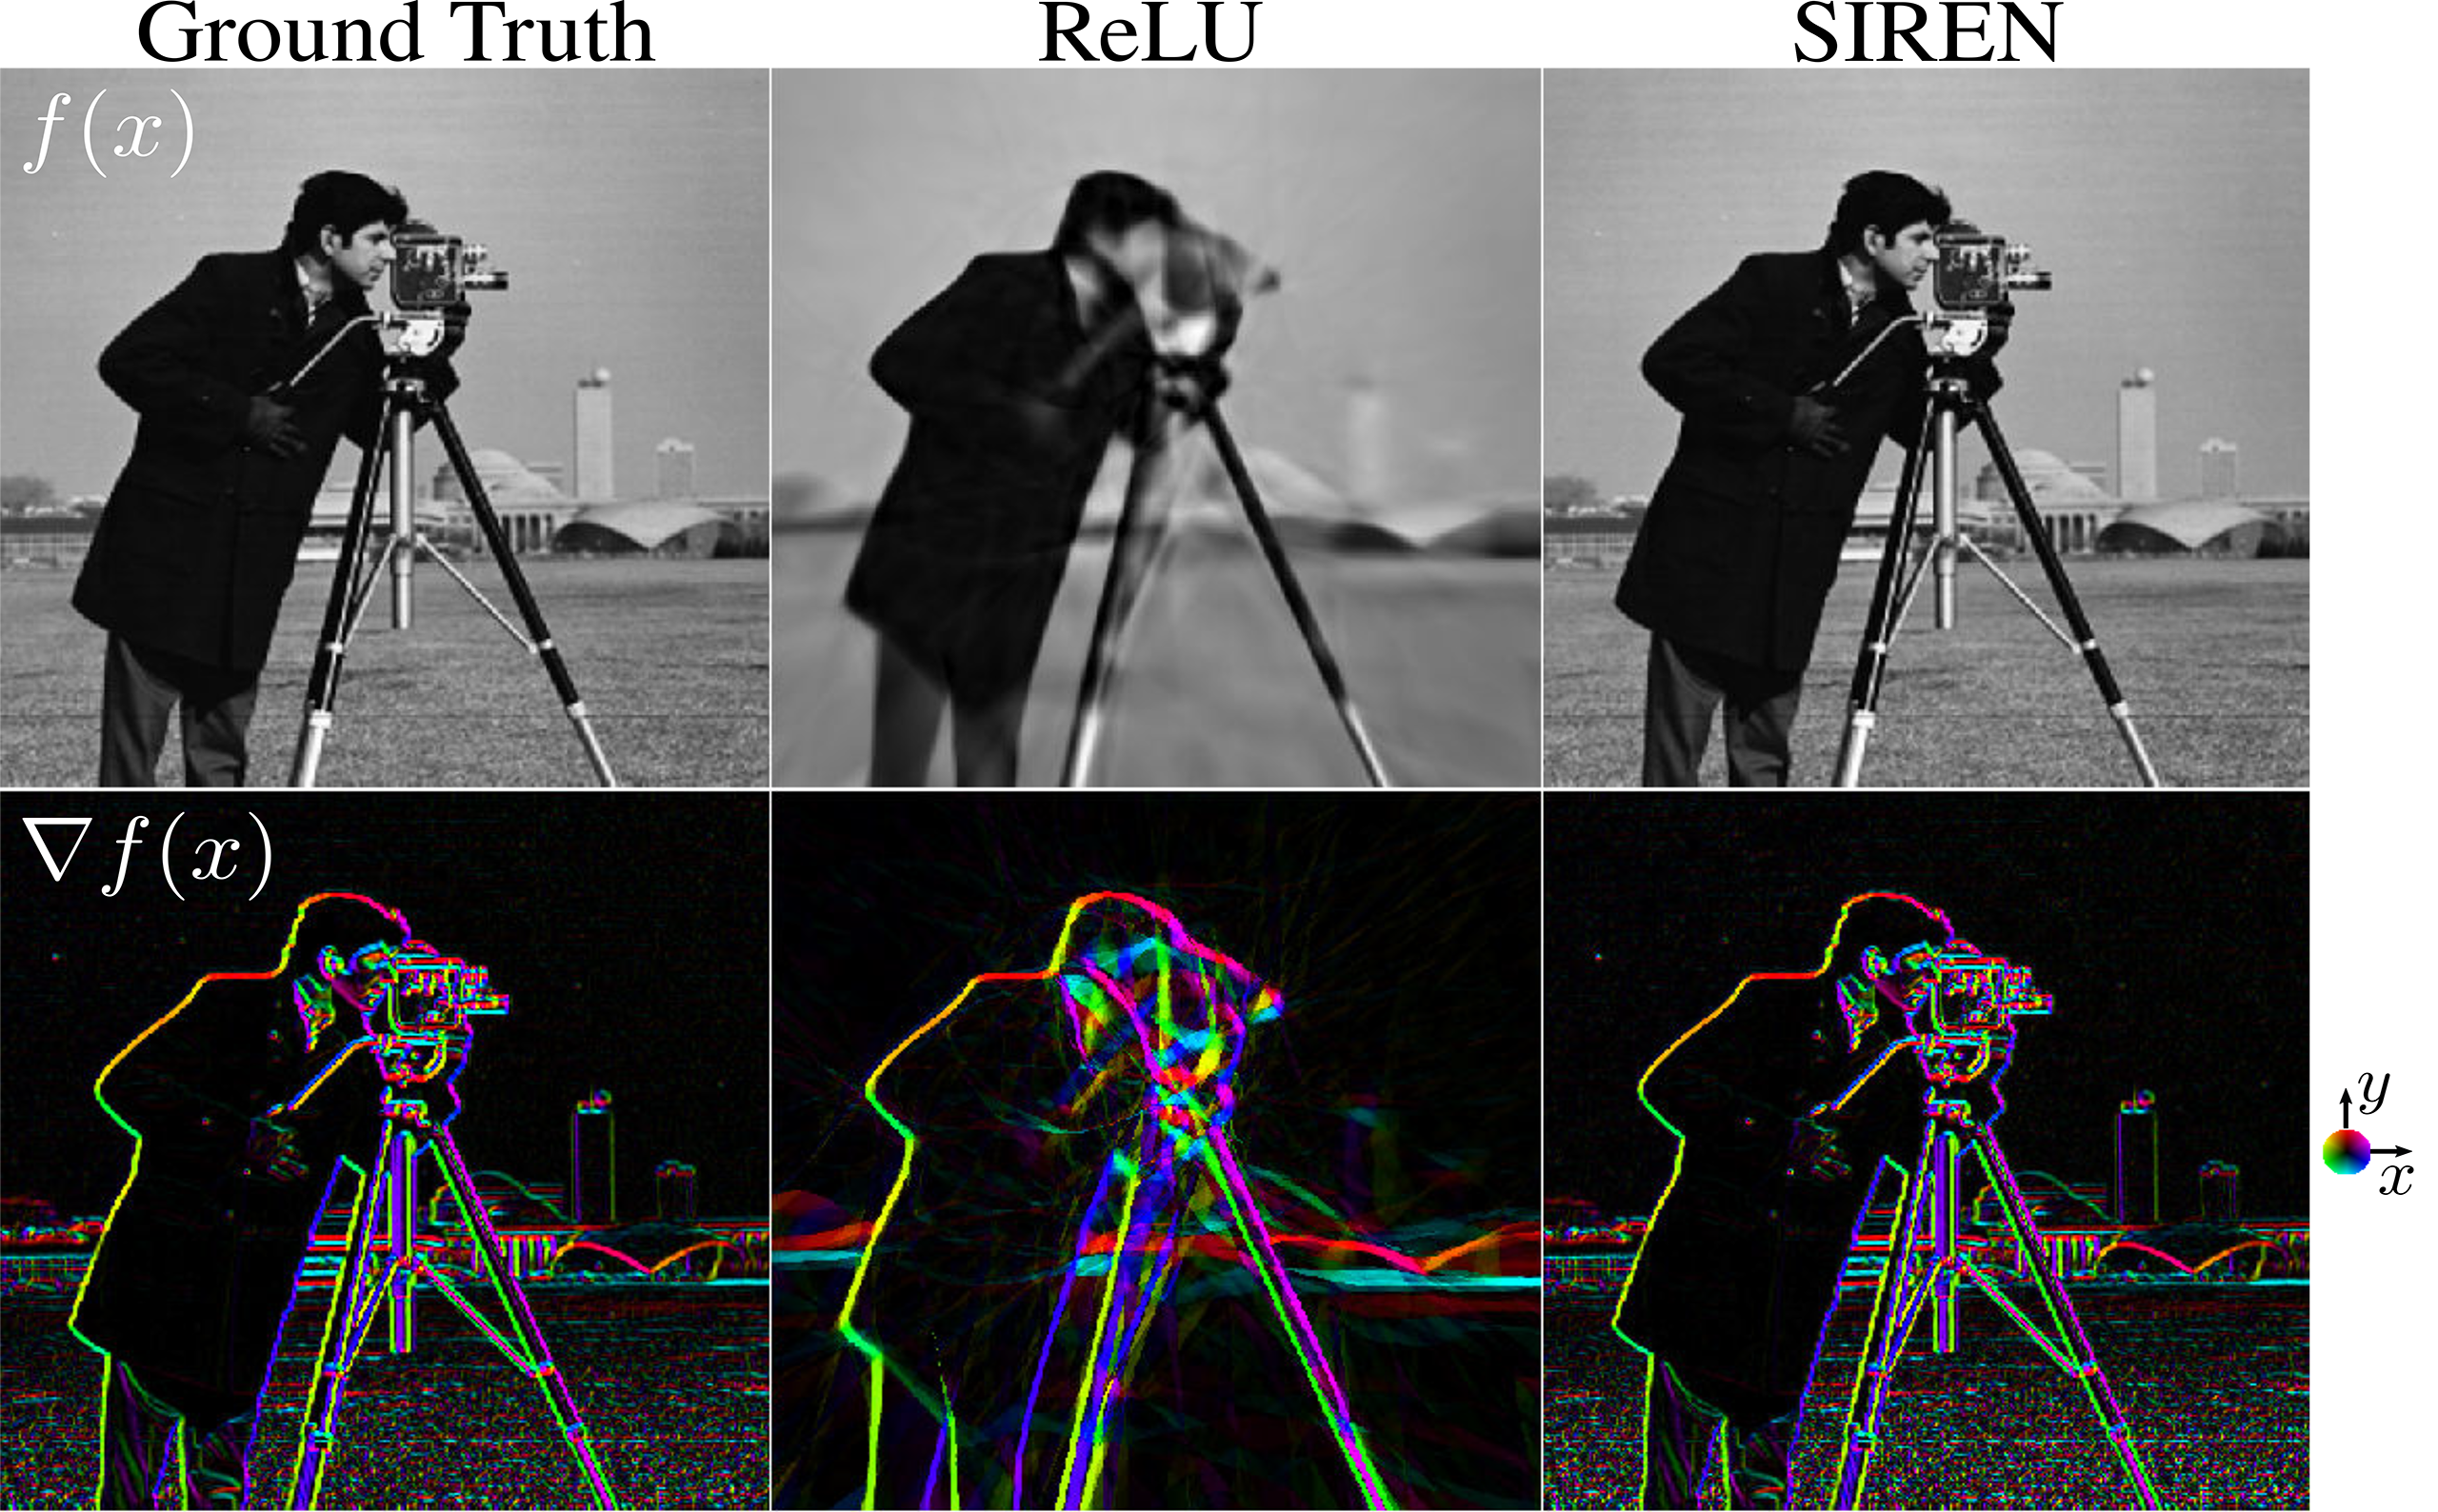
\includegraphics[width=0.6\linewidth]{Siren.png}
  \caption{激活函数对比\cite{sitzmann2020implicit}}
  \label{fig:siren_compare}
\end{figure}

实验\cite{sitzmann2020implicit}表明,采用正弦激活的MLP在3D形状重建任务中可将PSNR提升3-5 dB。
这一突破性进展验证了激活函数的频谱特性对于隐式神经表示质量的关键作用,同时为物理场仿真、
偏微分方程求解等需要高阶导数连续性的任务提供了新的解决方案。

\subsection{损失函数}
【】马上写。

\subsection{自动编码器} \label{sec:auto_encoder}
自动编码器(Autoencoder)作为深度学习中重要的无监督学习架构,其核心思想源于对生物感知系统中信息压缩与重建机制的仿生模拟。
该架构由对称的编码器(Encoder)与解码器(Decoder)网络构成,通过最小化输入数据与重建输出之间的差异,
迫使网络学习数据本质特征的紧凑表示。从数学角度来看,自动编码器可以看作是一种将高维数据转换为低维表示的工具:
编码器 $\mathcal{E}:\mathcal{X}\rightarrow\mathcal{Z}$ 将输入数据 $x\in\mathbb{R}^D$ 投影至 $z\in\mathbb{R}^d$ ,
解码器 $\mathcal{D}:\mathcal{Z}\rightarrow\mathcal{X}$则试图从潜在编码重构原始输入 $\hat{x}=\mathcal{D}\left(\mathcal{E}\left(x\right)\right)$,
其优化目标可以由公式\eqref{eq:ae_loss}给出:
\begin{equation}\label{eq:ae_loss}
\min_{\theta,\phi}E_{x\sim p_{\mathrm{dt}}}\Bigl[\bigl|x-\mathcal{D}_\phi\bigl(\mathcal{E}_\theta(x)\bigr)\bigr|^2\Bigr]
\end{equation}
其中$\theta$和$\phi$分别代表编码器与解码器的参数。这种方法不仅能在没有标注的数据中发现内在结构,而且在特征提取、
降维和去噪等应用中取得了很好的效果。早期的研究\cite{Hinton_2006}发现,当网络使用非线性激活函数并对低维空间进行一定限制时,
其能够有效地提取数据中的关键因素,比如在图像处理中自动识别边缘、纹理等重要视觉元素。

同时,自动编码器在处理复杂的光照估计与可微渲染问题时也有重要的作用。自动编码器的优势在于能够从高维数据中提取出最关键的特征,
并捕捉数据内在的低维结构。当我们面对真实世界的光照环境时(例如256\times256分辨率的环境贴图),
传统方法直接在原始像素空间进行优化会遇到三个问题:其一,像素数可能高达数百万,导致梯度下降等优化算法容易陷入局部最优;
其二,光照参数需要符合辐射度非负、能量守恒等物理规律,而仅仅依靠人工设计的正则项通常难以完全表达这些约束;
其三,实际光照中存在一些低维特性(如色温分布、主要光源的方向偏好),但要显式建立这些规律需要精确的先验知识。

因此,在可微渲染的任务里,自动编码器能够利用数据压缩的特性,通过编码器将高维环境贴图压缩到一个较低维的潜在空间,
构建出紧凑的光照参数表示,从而大大降低了优化问题的维度。同时,解码器将潜在向量映射回满足物理规律的光照配置,
确保优化过程中始终处于可行解范围内。这种“压缩-重建”机制实际上学习了一个数据驱动的光照投影操作,使得光照估计问题可以转化为在一个
平滑且低维的空间中进行高效搜索。例如,在同时优化物体材质和光照时,只需要调整潜在空间中的少量参数,就能获得物理上合理的光照重构,
而无需直接处理数百万维的像素数据。

\section{传统渲染管线}
本节介绍传统渲染管线的相关知识,为本文针对工作流进行光照分解补充相关背景知识。传统渲染管线中,
数字资产通常由网格体和多张纹理贴图组成,其中,网格体表达了数字资产的几何形状,纹理贴图和各类参数表达了数字资产表面不同的光学属性。
本节将介绍数字资产的制作和渲染过程,并解释数字资产与着色模型之间存在的耦合关系。

\subsection{渲染方程}


渲染方程(Rendering Equation)是计算机图形学中描述光与物体表面交互的基础方程之一。
由Kajiya等人于1986年提出\cite{Kajiya_1986},它为物体表面的光照计算提供了一个物理上合理的模型,
广泛应用于真实感渲染和计算机图像生成中。渲染方程通过描述光从场景中的光源到达表面并反射到观察者的过程,
计算表面点的辐射亮度(radiance)。具体计算过程如公式\eqref{eq:rendering_equation}:
\begin{equation}
  \label{eq:rendering_equation}
  L_o\left({\bf{x}},\omega_o\right)=\int_{\upOmega}f_r\left({\bf{x}},\omega_i,\omega_o\right)\cdot L_i\left({\bf{x}},
  \omega_i\right)\left(\omega_i\cdot\mathbf{n}\right)\,\mathrm{d}\omega_i
\end{equation}
其中,$L_o\left({\bf{x}},\omega_o\right)$表示从表面点$\bf{x}$沿观察方向$\omega_o$看到的辐射亮度,
$L_i\left({\bf{x}},\omega_i\right)$是从入射方向$\omega_i$到达表面点$\bf{x}$的光源辐射亮度,
$f_r\left({\bf{x}},\omega_i,\omega_o\right)$是BRDF,
它决定了光线从入射方向$\omega_i$到反射方向$\omega_o$的散射方式,且依赖于表面的材质属性。
$\left(\omega_i\cdot\bf{n}\right)$表示入射光与表面法线$\bf{n}$的点积,代表表面与光源的接触程度,
而$\mathrm{d}\omega_i$是入射光方向的微小立体角元素。

渲染方程的核心思想是通过积分所有可能的光源对表面反射的贡献,计算出最终的观察光照。
其在实际应用中能够模拟多种光照现象,包括漫反射、镜面反射、折射以及其他复杂的光学效应。
然而,尽管渲染方程具有强大的表达能力,但其高计算成本使得在实时渲染中难以直接应用。
因此,许多基于渲染方程的模型需要进行简化或近似,以实现高效的图像生成。

\subsection{着色模型}

着色模型(Shading Model)是基于渲染方程的简化或近似,通常用于图形学中的实时渲染。其主要目标是通过简化光的反射过程,
使得渲染计算更加高效。通过引入一定的数学公式和参数设置,着色模型能够近似真实世界中的光照现象,
从而生成具有理想真实感或艺术效果的图像。着色模型的核心是描述光线与物体表面相互作用的数学函数,
输入通常包括入射光线、视角、表面法线以及材质属性(如漫反射颜色、镜面反射强度、粗糙度等),
输出则是某一点处的最终光照颜色或亮度。常见的着色模型包括:

\fourthtitle{1}基于物理的着色模型

这些模型遵循物理定律,精确描述光照现象,通常依赖于双向反射分布函数。
例如,Cook-Torrance模型[29] 通过微表面分布函数、几何遮蔽因子和Fresnel反射等参数,精确地模拟了金属和非金属表面的反射行为。
基于物理的着色模型能够较为准确地模拟光的反射、折射和散射过程,生成更为真实的视觉效果。

\fourthtitle{2}经验性(非物理)着色模型

这类模型通常采用简化或经验公式来近似光照计算,
代表性的有Blinn-Phong模型和Lambertian模型。尽管它们并不完全遵循物理定律,
但通过经验参数(如光泽度、反射系数等)的调控,依然能够生成具有一定真实感的光照效果。
由于计算复杂度较低,经验性模型广泛应用于实时渲染或资源受限的场景。

\subsection{工作流}
工作流(Workflow)在计算机图形学中指的是一套标准化的参数与贴图生成流程,它定义了如何结合和组合各类材质参数和贴图,
以表述数字资产表面不同的光学属性。简言之,工作流决定了如何构建数字资产的表面属性,使其能够符合特定的着色模型的计算需求。
因此,选择适当的工作流对于高效且精准地表达材质的视觉效果至关重要。

工作流与着色模型之间具有紧密的耦合关系,每种工作流设计都对应着特定的着色模型,这些模型通过接收由工作流生成的参数和贴图,
进行光照计算与视觉效果渲染。不同的工作流基于不同的物理或经验性模型,表达表面特性的方式也有所不同。
本节介绍三种工作流兼具了基于物理的以及非物理的着色模型,并且仍在现代渲染引擎和项目中广泛使用。

\fourthtitle{1}金属度工作流

该工作流利用金属度(Metallic)贴图区分金属与非金属区域,使用粗糙度(Roughness)描述表面的粗糙程度。
由于该工作流直接描述物体表面的金属性质,因此渲染效果更易符合预期。在该工作流的数字资产中,共使用三张纹理:
基础色(Albedo)纹理在金属材质中表示镜面反射颜色,而在非金属中表示漫反射颜色,记为$\mathbf{b}$;
金属度(Metallic)贴图区分金属与非金属区域,记为$m$;粗糙度(Roughness)描述表面的粗糙程度,记为$r$。

金属度工作流可以使用微表面模型的Cook-TorranceBRDF完成计算,该模型将渲染方程中的$f_r$分为漫反射项$f_d$
以及高光反射项$f_s$:
\begin{equation}\label{eq:cook-torrance}
f_r=f_s+f_d.
\end{equation}

漫反射项$f_d$表示表面上从所有方向散射的光,通常使用Lambertian反射模型表示,即光照强度与表面法线和入射光方向的夹角无关,
只与入射光的方向有关,计算过程如下:
\begin{equation}\label{eq:lambertian}
f_d=\frac{1-m}{\pi}
\end{equation}

高光反射项$f_s$表示光线在光滑表面上按镜面反射规律反射的部分,通常依赖于入射光和观察方向与表面法线之间的角度关系,
可以被表示为:
\begin{equation}\label{eq:specular}
f_s(\omega_o,\omega_i)=\frac{D({\bf{h}};r)\cdot F(\omega_o,{\bf{h}};{\bf{b}},m)\cdot G(\omega_i,\omega_o,{\bf{h}};r)}
{4\cdot({\bf{n}}\cdot\omega_i)\cdot({\bf{n}}\cdot\omega_o)}
\end{equation}

其中,$D$是法线分布函数(Normal Distribution Function, NDF),$F$是菲涅尔(Fresnel)反射项,$G$是几何遮蔽(Geometry)
项,$\bf{h}$是半角向量,$\bf{n}$为表面法线。针对$D$项、$F$项以及$G$项的计算,不同的研究中针对着色风格均提出了多种实现,
接下来本文将介绍主流的几种计算方法。

在大多数渲染器中,$D$项通常使用GGX\cite{walter2007microfacet}计算,使用粗糙度控制其锐利程度:
\begin{equation}\label{eq:D_ggx}
D({\bf{h}};r)=\frac{r^2}{\pi\Bigl(({\bf{n}}\cdot{\bf{h}})^2(r^4-1)+1\Bigr)^2}
\end{equation}

同时,为了在可微渲染中使用,$D$项也可以由球面高斯(Spherical Gaussians)近似计算为:

\begin{equation}\label{eq:Dsg}
D_{\rm{SG}}({\bf{n}};r)=\frac{1}{\pi r^4}\exp\Biggl(\frac{2}{r^4}\Bigl({\bf{n}}\cdot{\bf{h}}-\mathbf{1}\Bigr)\Biggr)
\end{equation}

F项可以根据Schlick等人\cite{schlick1994inexpensive}的研究近似计算,由如下公式给出:
\begin{equation}
  \label{eq:F}
  F(\omega_o,{\bf{h}};{\bf{b}},m)=F_0+\bigl(1-F_0\bigr)\Bigl(1-(\omega_o\cdot{\bf{n}})^5\Bigr)
\end{equation}
其中,$F_0$ 项可以通过公式\eqref{eq:F_0}表示为:
\begin{equation}
  \label{eq:F_0}
  F_0=0.04(1-m)+{\bf{b}}m
\end{equation}

最后,G项可以根据Heitz等人\cite{heitz2014understanding}的研究使用Smith联合遮蔽阴影函数(Smith Joint Masking-Shadowing),计算方式如下:
\begin{equation}
  \label{eq:G}
  G(\omega_i,\omega_o,{\bf{n}};r)=G_{\rm{GGX}}(\omega_i\cdot{\bf{n}})\,G_{\rm{GGX}}(\omega_o\cdot{\bf{n}})
\end{equation}
其中,$G_{\rm{GGX}}$ 由公式\eqref{eq:G_ggx}计算:
\begin{equation}
  \label{eq:G_ggx}
  G_{\rm{GGX}}(z)=\frac{2z}{(2-r^2)z+r^2}
\end{equation}

\fourthtitle{2} Specular工作流

该工作流通过镜面反射(Specular)贴图和漫反射(Diffuse)贴图直接控制材质表面的镜面反射与漫反射颜色,
通过光泽度(Glossiness)贴图控制镜面反射的强度和大小。Specular工作流与描述表面物理性质的Metallic工作流不同,
该工作流更为灵活,可以为材质单独指定不同的镜面反射率。例如蓝色的陶瓷材质对于Metallic工作流可能需要设置部分违反物
理直觉的值才能实现,但是使用Specular工作流时可以直接调整出真实的反射表现。

在计算上,Specular工作流也使用Cook-Torrance BRDF,区别在于部分计算方式不同。首先,对于上文中公式\eqref{eq:F}所述的菲涅尔项$F$,
Specular工作流替换了其中的$F_0$:
\begin{equation}\label{eq:F0_spec}
F_0=\bm{c}_s
\end{equation}
随后,在计算漫反射项$f_d$时不再根据金属度进行插值,而是使用菲涅尔项$F$作为插值系数:
\begin{equation}\label{eq:diffuse_spec}
f_d=\frac{1-F}{\pi}
\end{equation}
这种计算方式使得即使Specular允许艺术家自由分配镜面反射和漫反射的表现,也保证了能量守恒,尽量避免出现物理不真实的问题。

\fourthtitle{3} Blinn-Phong工作流

该工作流基于经验性着色模型(Blinn-Phong模型),通常依赖漫反射(Diffuse)、高光反射(Specular)贴图来模拟光照效果。其中高光反射参数在公式中实现了高光部分的近似计算,以光斑的形式提供近似的光滑观感,高光反射项$f_s$计算方式如下:
\begin{equation}\label{eq:specular_BlinnPhong}
f_s=\max(\mathbf{n}\cdot \mathbf{h},0)^\alpha
\end{equation}
漫反射部分使用Lambertian经验模型。总体的计算方式可以通过如下公式表示:
\begin{equation}\label{eq:diffuse_BlinnPhong}
f_d=\frac{1}{\pi}
\end{equation}

尽管该工作流并不严格遵循物理法则,且渲染效果无法与基于物理的模型相比拟,但它的计算开销较小,无需复杂的积分,适合用于对渲染效率有较高要求且对真实感要求较低的项目,非常适合于手机等移动端设备。

\subsection{数字资产与着色模型的耦合}
从前文的介绍可以看出,数字资产与着色模型之间存在着紧密的耦合关系。每种工作流预设了特定的参数组织方式,
并且与相应的着色模型或反射模型密切绑定。例如,金属度工作流通常与基于物理的Cook-Torrance BRDF模型配合使用,
以确保在渲染时,金属与非金属材质在光照下的反射行为符合物理规律。如果工作流中预设的参数与着色模型所需的参数不匹配,
可能导致最终渲染结果与预期不符,进而影响数字资产的效果和视觉质量。

尽管这种耦合关系使得数字资产的制作流程更加直观,并且提高了资产制作的效率与规范性,但它也存在一定的局限性。
特别是在开发过程中,这种严格的绑定要求数字资产必须按照特定规范进行制作,从而限制了技术迭代的灵活性。
在一些大型项目或长期维护的项目中,若需要升级着色模型,通常会导致大量现有数字资产需要重新制作或手动转换,
消耗了巨大的时间和经济成本。

为了解决这一问题,本文提出了一种新的解决方案:设计并实现一套端到端的数字资产管线,
通过将数字资产表示为神经辐射场(NeRF),并根据指定的工作流进行分解,从而打破数字资产与着色模型之间的紧密耦合。
该管线能够使数字资产在保持物理准确性和艺术效果的同时,具有更高的灵活性和可扩展性,进而为着色模型的快速迭代和工作流的适配提供支持。

\section{可微渲染理论基础}
传统渲染过程将三维场景描述转换为二维图像,但在标准计算机图形学管线中,该过程通常是不可微的,
如遮挡判断与离散三角形选择的操作并不连续,导致难以获得有效的梯度信息。
这一特性限制了渲染在基于梯度优化的机器学习和计算机视觉任务中的应用。
可微渲染(Differentiable Rendering, DR)是一种将传统渲染过程与梯度优化方法相结合的新兴技术,
其核心理念是致力于实现从三维场景到二维图像的映射过程中的可微性,从而能够通过误差反向传播直接优化场景参数。
因此,这一技术在计算机视觉和三维重建等任务中具有重要价值。

可微渲染的核心目标是计算渲染图像相对于场景参数的梯度,即$\tfrac{\partial I}{\partial \upPhi}$,
其中$I$是渲染图像,$\upPhi$包含几何、材质、光照和摄像机参数。由于渲染过程中的某些操作(如光栅化、可见性计算和光照建模)
通常具有离散性或复杂的非线性特性,使得计算其导数较为困难,不同的可微渲染方法针对这些挑战提出了解决方案。
接下来,本文将分别介绍可微渲染中常见的光照表示技术和几何形状表示方法。

\subsection{基于图像的照明与近似}
可微渲染中的光照表示需要满足多个关键需求,包括精确性、可微性以及对复杂光照环境的高效建模。
在这一背景下,基于图像的光照(Image Based Lighting, IBL)技术成为广泛应用的选择。
在完整的渲染方程\eqref{eq:rendering_equation}中,常规离散光源被表示为$L_i(\mathbf{x},\omega_i)$,
其在计算时需要考虑着色点的位置,而在IBL中则假设环境处于“无限远”状态。也就是说,
任何一处的光源所发出的光线都是平行的,而且其辐射强度在空间中是均匀的。这种假设使得对于场景中任何一点,
入射光的强度仅依赖于光线的方向,而不依赖于具体的位置,仅需计算$L_i(\omega_i)$

此外,可微渲染需要光照模型在物理上保持连续性,从而支持梯度的计算与传播。IBL采用环境贴图存储光照数据,
通过球面投影方式在空间中形成自然的连续分布。相比离散的点光源,环境贴图能够以较高的分辨率捕捉光照场景中的细节,
同时在可微渲染的优化过程中避免了不连续性对梯度的影响。这种连续性确保了光照参数的可导性,
从而能够在可微渲染中有效优化与光照相关的参数。

除此之外,Hill等人\cite{Hill_2014}引入了分裂和近似(Split-Sum Approximation),并将其应用于现代即时渲染中,以进一步降低计算量。
分裂和近似方法主要目的是将原本公式\eqref{eq:rendering_equation}中需要在半球上计算的高维积分
拆分成两个易于预计算并在运行时快速查表获得的部分,从而大大降低计算成本,
同时获得足够精确的视觉效果。分裂和近似的思想可以由公式\eqref{eq:int_approx}表示:

\begin{equation}
  \int f(x)g(x){\rm{d}}x\approx \int{f(x){\rm{d}}x} \int{g(x){\rm{d}}x}
  \label{eq:int_approx}
\end{equation}

公式\eqref{eq:int_approx}将两个函数乘积的积分近似为两个函数积分的乘积,
当该思想应用于渲染方程中的镜面反射项时,则镜面反射项可以通过以下形式近似计算:

\begin{equation}
  L(\omega_o)\approx 
  \int_{\upOmega}{f(\omega_i\cdot{\bf{n}}){\rm{d}}\omega_i}
  \int_{\upOmega}{L_i(\omega_i)D(\omega_i,\omega_o)(\omega_i\cdot{\bf{n}}){\rm{d}}\omega_i}
  \label{eq:L_omega_o_approx}
\end{equation}

其中,第一项表示白色环境光照的镜面BSDF积分,取决于参数$\cos{\theta}=\omega_i\cdot{\mathbf{n}};$
第二项表示法线分布函数与入射光的积分,当采用环境贴图技术时,该项可以被视作按照不同的表面粗糙度对环境贴图进行过滤,
也可以通过Mipmap等技术预先进行计算。通过IBL技术以及分裂和近似,着色时的计算量得以大幅减少,
因此这两项技术对于可微渲染任务来说不可或缺。

但是,IBL技术在实现过程中依赖的假设简化了光照建模的复杂性,将环境光表示为来自球面上的均匀方向分布,
而忽略了光源与场景之间的距离关系、遮挡关系。这种假设在许多传统渲染任务中是合理的,但在可微渲染中,
这种假设限制了IBL对光照空间分布的表达能力,尤其在涉及局部光照变化的场景中。例如,在阴影区域中,
光线受到物体遮挡后显著衰减,而IBL由于假定光照均匀分布于无限远,难以精确捕捉遮挡效应,
从而导致阴影处的光照表示不准确。此外,IBL的假设忽略了离散光源直接光的影响,无法精确建模光源位置与着色点之间的几何关系。
因此,在传统渲染中由点光源或聚光灯直接形成的高频光照效应(如强烈的高光或投影)也难以通过IBL实现。

\subsection{几何表示}
几何表示是可微渲染的关键组成部分, 用于描述场景的几何形状。用于可微渲染的良好几何表示应该捕获
局部几何细节并表示具有任意拓扑的对象,同时还具有内存和计算效率,以便在交互式应用程序中进行快速推理。
根据实现原理,表示形式主要可以分为传统图形学中的显式表示和结合了深度学习和神经网络的隐式表示两类。

\fourthtitle{1} 显式表示

显式表示方法通过直接定义物体表面的几何元素实现对三维形状的描述,主要包括网格(Mesh)、点云(Dense Cloud)
和符号距离函数(Signed Distance Function, SDF)三种典型形式。其中,网格表示通过顶点、边和面构成的多边形网格刻画物体形状,
其顶点可附加纹理坐标、法线及颜色等属性,具有直观可编辑的特点,且能高效利用图形硬件的加速能力。
然而,实际应用中不同存储格式的兼容性问题常需额外处理,且网格拓扑结构的刚性约束限制了其在重建任务中对高频细节的还原能力。
点云表示通常由激光扫描或立体视觉设备直接生成,具有采集便捷、密度可调的优势,但因缺乏显式拓扑关联,
其直接渲染效果粗糙且编辑灵活性不足,难以满足高质量实时交互需求。
相比之下,符号距离函数(SDF)通过为空间点赋予到表面的带符号距离值,既能以连续函数形式捕捉几何细节,
又可实现紧凑的数据存储,但其计算复杂度与空间分辨率的关系需通过特定算法优化。

\fourthtitle{2} 隐式表示

隐式表示通过参数化模型间接定义几何形状,近年来以神经隐式表示为核心的研究取得了显著进展。
该类方法利用神经网络$F(P_i^{xyz})$预测三维点$P_i^{xyz}\in\mathbb{R}^3$的几何属性,
其内存消耗与空间分辨率无关,理论上支持无限分辨率的表面重建。典型实现包括三种范式:
占据概率模型将几何描述转化为二分类问题,通过神经网络预测点$P_i^{xyz}$位于物体内部的概率以定义形状边界;
透明度建模则直接学习空间点的透明属性,既可表征半透明物体,也可近似非透明体的占据概率;
水平集方法将物体表面定义为隐式函数$F(P_i^{xyz})=0$的解集,通过距离函数的符号区分内外空间,
在复杂几何重建中兼具精度与计算效率优势。尽管神经隐式表示存在训练耗时、采样效率低等挑战,
但其参数化特性与拓扑无关性为高精度复杂几何建模提供了突破性解决方案,
尤其在细节还原和动态拓扑适应方面展现出独特潜力。

\fourthtitle{3} 混合表示
现有的隐式神经表示方法难以将生成结果直接用于下游编辑等任务,而传统的显式网格体在重建效果上有所折损,
而Shen等人\cite{shen2021deep}提出了深度行进四面体(Deep Marching Tetrahedra,DMTet),
该方法结合了SDF与网格体表示的优点,并且计算过程可微,适用于可微渲染管线。

DMTet使用离散的SDF表示每个顶点相对于原位置的偏移量,通过可微行进四面体层
(Differentiable Marching Tetrahedra Layer,MT)将SDF转换为三角形网格,
使得该技术能够基于SDF进行优化,并直接转换为网格体。由于这种转换能够在网络优化期间进行,避免了
传统隐式表示在管线后额外转换为网格表示时引入误差的情况。同时,DMTet也解决了直接使用网格体进行优化时,
网格体拓扑相对固定、无法表示细微高频细节的情况。

DMTet的优化过程如下,当给定一个四面体网格(Tetrahedral Grid),对于网格中的每个顶点v,
DMTet学习对应的SDF值$s$和变形向量$\Delta\mathbf{v}$,随后根据学习到的SDF值生成三角形面,
构成网格体。

DMTet从SDF生成三角形面的计算方式如图\ref{fig:dmtet_calc}所示,其中,标量$s$表示SDF值,
顶点$v_i$的位置$v_i^\prime$根据$s_i$的偏移进行更新,两个相邻顶点$v_i$和$v_j$之间的顶点$v_{ij}$通过线性插值进行计算。

\begin{figure}[htbp]
  \centering
  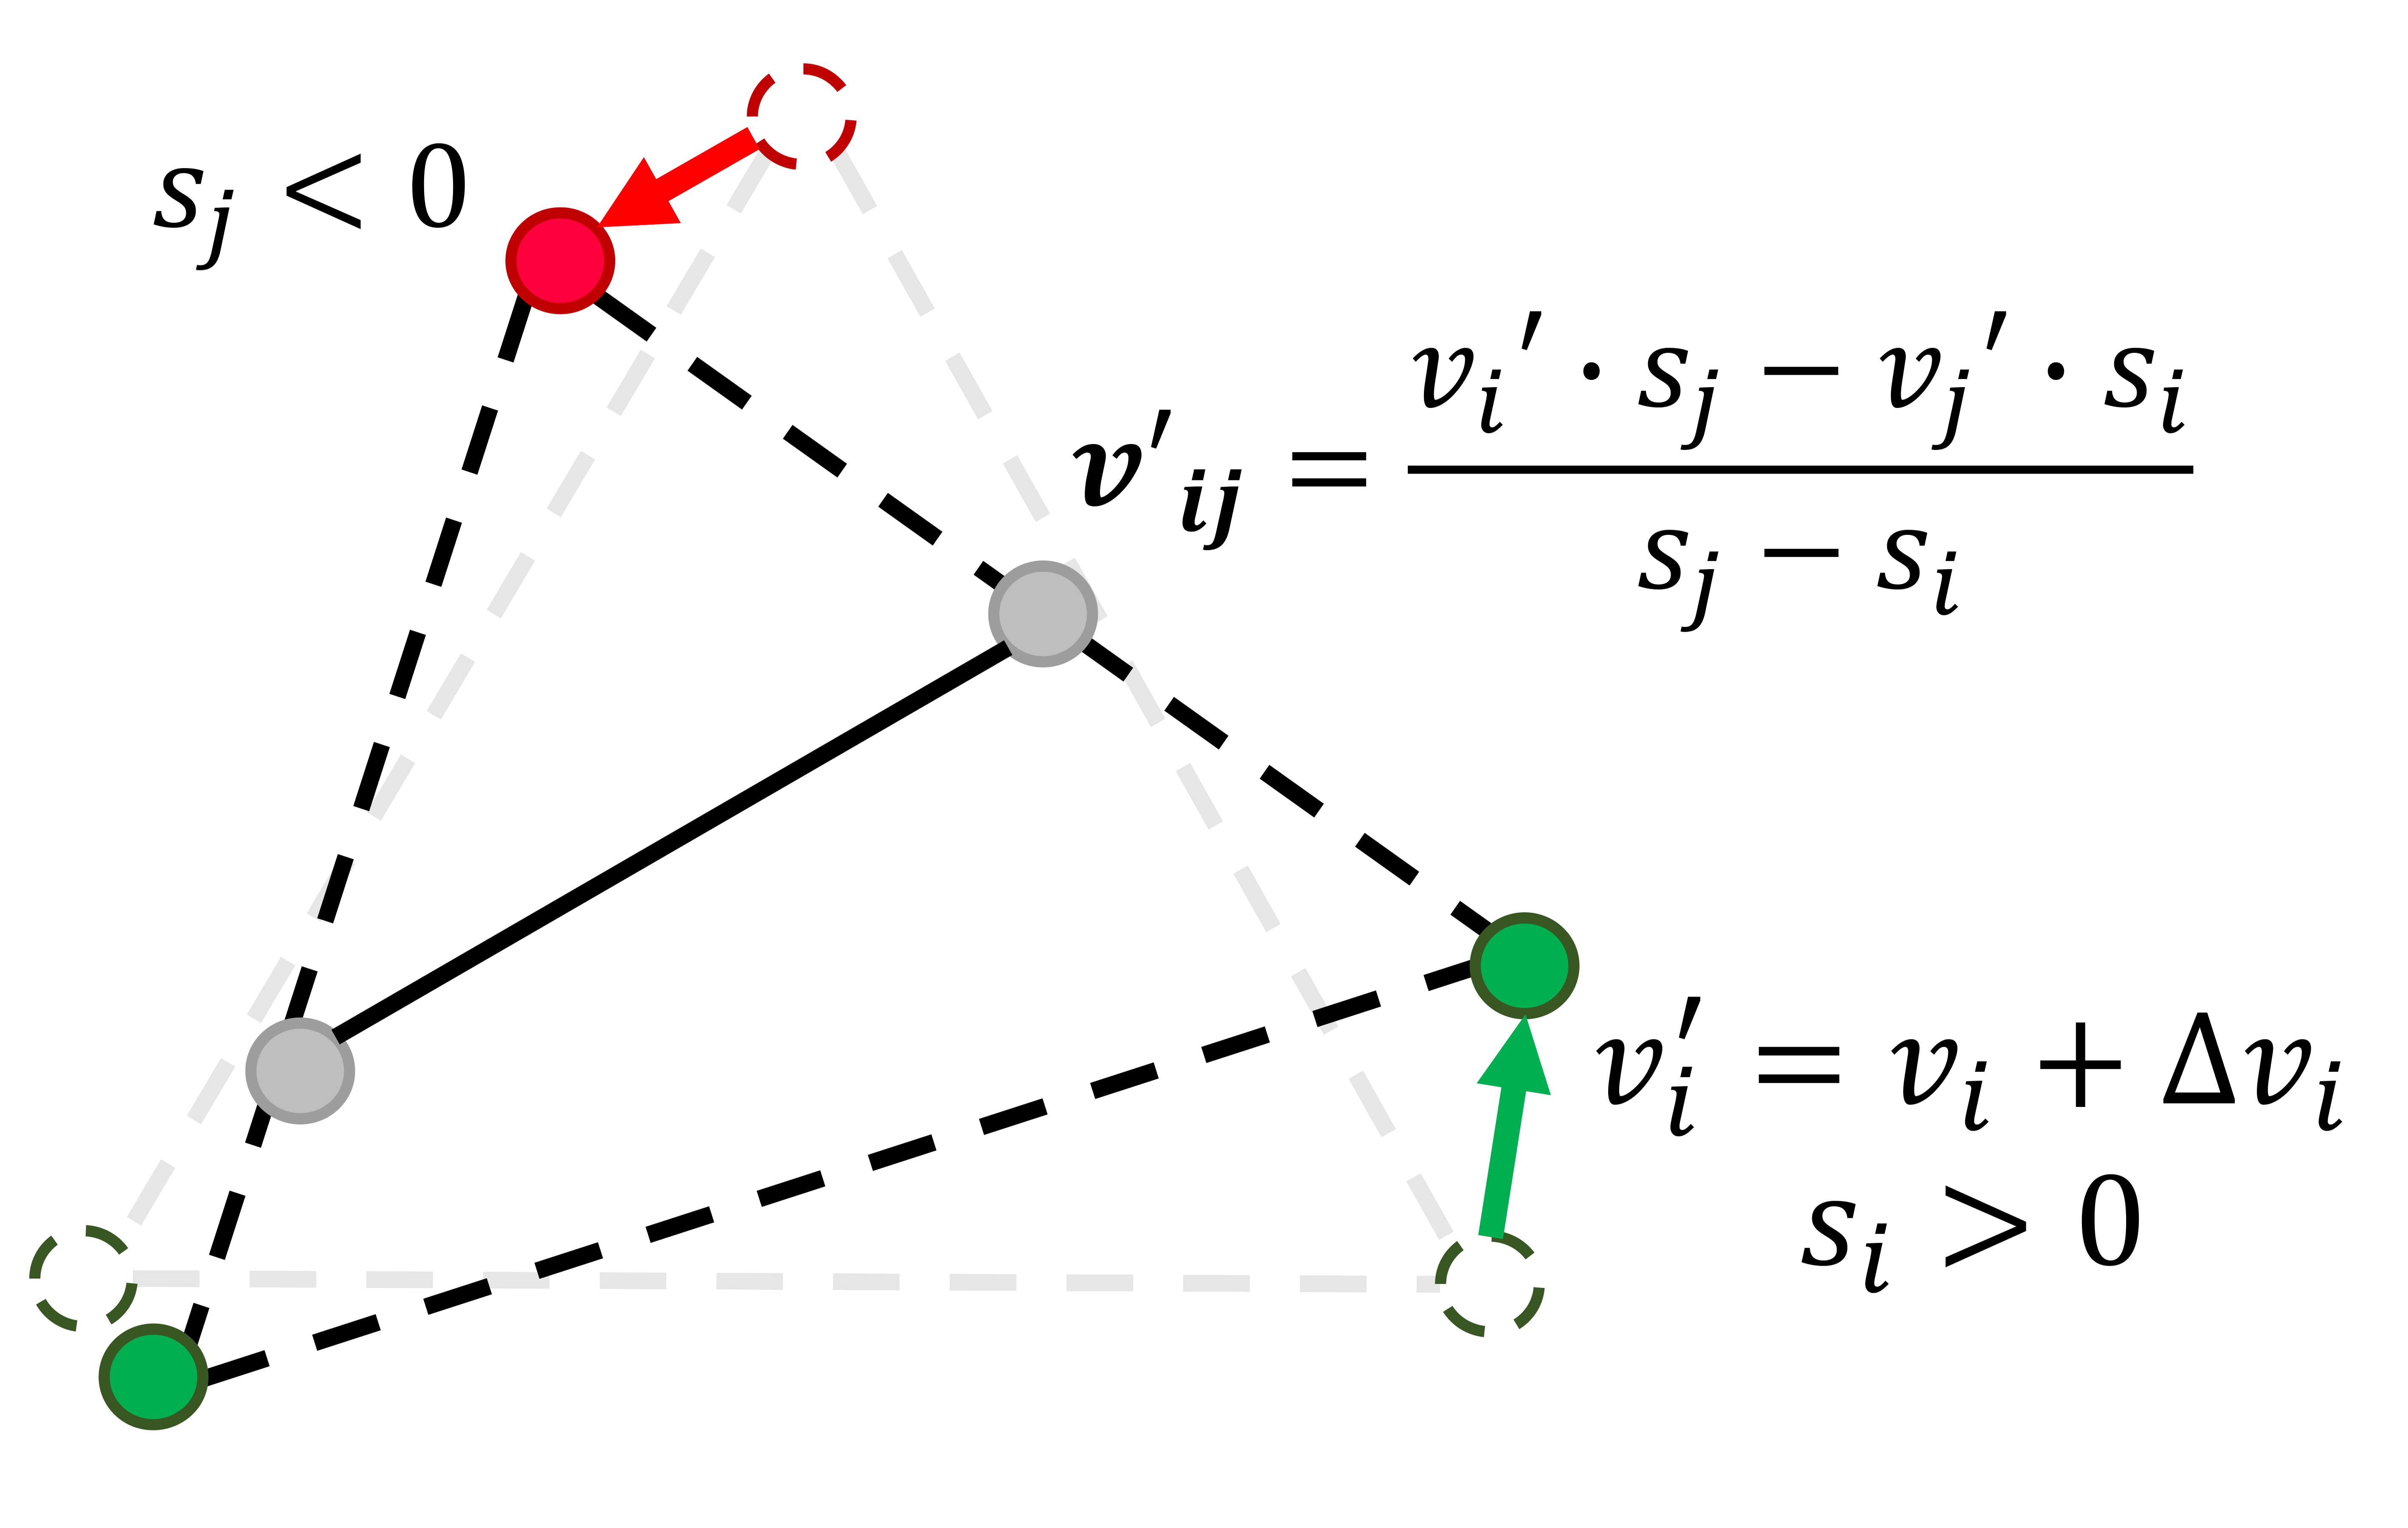
\includegraphics[width=0.5\textwidth]{SDFtoMesh.png}
  \caption{DMTet计算三角形面的过程}
  \label{fig:dmtet_calc}
\end{figure}

\section{NeRF理论基础}

NeRF技术通过融合辐射场建模与可微分体积渲染,实现了仅凭多视角二维图像即可优化三维场景隐式表示的技术突破。
作为基于坐标的多层感知机在视觉任务中的扩展,NeRF通过分析一组从多个视角捕获的二维图像,
能够推断出场景的三维几何结构和视觉外观。这种方法的核心优势在于其能够合成全新的视角图像,
即便这些视角在原始图像集中并未直接观测到。NeRF技术的突破性在于它对光线在三维空间中的传播进行建模,
利用深度神经网络学习和推理光线与物质相互作用的复杂过程,从而实现对场景的髙度真实感渲染。
这不仅在计算机视觉领域引起了革命性的变革,也为图形学的发展开辟了新的研究方向。
本章节将详细介绍神经辐射场的基本理论框架、关键技术要点,提供一个全面深入的技术解析。

\subsection{NeRF的基本定义}
NeRF作为计算机视觉领域的一项前沿进展,延续了基于坐标的多层感知机以空间坐标为输入的基本架构,
但其建模对象从单一几何属性升级为辐射场函数。NeRF的基本原理是通过深度学习将三维空间中的点映射到其对应的颜色和密度,
本身的功能可以用公式\eqref{eq:nerf_mapping}定义:

\begin{equation}
  F_{\upTheta}:({\bf{x}}, {\bf{d}})\rightarrow({\bf{c}},\sigma)
  \label{eq:nerf_mapping}
\end{equation}

其中,$\mathrm{x}\in\mathbb{R}^3$表示三维场景内的坐标,$\mathrm{d}\in\mathbb{S}^\mathbf{2}$
表示观察方向的方位角和极角,$\mathrm{c}\in\mathbb{R}^3$表示场景在$\mathrm{x}$点、于观察方向$\mathrm{d}$
进行观察时的RGB颜色,$\sigma$表示场景在$\mathrm{x}$点的密度,物理意义该点为是否存在物质或光学吸收现象,
函数$F_{\upTheta}$由一个或多个MLP完成实现。NeRF的总体框架如图\ref{fig:nerf_pipe}所示。


\begin{figure}[htbp]
  \centering
  \includegraphics[width=1.0\textwidth]{NeRFPipe.png}
  \caption{NeRF训练和渲染过程\cite{Mildenhall_2020}}
  \label{fig:nerf_pipe}
\end{figure}

NeRF的基础结构使用了前文介绍的基于坐标的多层感知机,并利用公式\eqref{eq:fourier_encoding}表示的傅里叶变换对
输入坐标$\bf x$进行了位置编码,显著提升了NeRF对高频几何细节的重建能力。

\subsection{NeRF的体积渲染}

本节介绍如何通过NeRF通过观察方向$\bf d$计算输出像素颜色$\bf c$。
这一过程的核心是通过体积渲染(Volume Rendering)方法来合成二维图像。
体积渲染将沿着每条射线对函数$F_{\upTheta}$输出的颜色和密度进行积分,计算射线的最终输出颜色$\bf c$,该过程可以由以下公式表示:
\begin{equation}\label{eq:volume_rendering}
C=\int_{t_n}^{t_f}T(t)\,\sigma(r(t))\,{\bf c}(r(t),{\bf d})\,\mathrm{d}t
\end{equation}
其中,$t_f$和$t_n$分别代表沿着射线方向积分的起始和结束时刻。对沿方向$\bf{d}$发射的光线$r$,
其$t$时刻所到达的点为$r(t)$。$\bf{c}$是三维空间中给定点$r(t)$在观察方向为$\bf{d}$时的颜色,
$\sigma$是点$r(t)$的密度,颜色$\bf c$和密度$\sigma$由函数$F_{\upTheta}$计算。$T(t)$是从相机到$t$时刻位置的透射率,
$T(t)$的定义如下所示:
\begin{equation}\label{eq:transmittance}
T(t)=\exp\Biggl(-\int_{t_n}^{t}\sigma(r(s))\,\mathrm{d}s\Biggr)
\end{equation}

$T\left(t\right)$是体密度函数,$r\left(s\right)$是光线路径上的点。神经辐射场接受空间中点的坐标$\left(x,y,z\right)$
以及射线的出发点和方向作为输入,然后输出在该点的颜色和密度,对射线上所有采样点的颜色和密度进行积分求和,
即可得到最终成像图像对应像素的颜色和密度。

\subsection{衡量指标}

本节介绍与NeRF技术相关的一系列研究领域中,用来评估网络生成质量的常用衡量指标。

\subsubsection*{(1)峰值信噪比} 

峰值信噪比(Peak Signal-to-noise Ratio,PSNR)是一种基于均方误差(Mean-square Error,MSE)
来计算图像之间绝对差异的方法,其计算过程简单直观,能够有效反映图像重构过程中细节信息的丢失或噪声引入问题,
PSNR的高低直接揭示了光照输出图像与原始真实图像在整体灰度层面上的恢复效果。
因此,PSNR能够为本文方法的有效性提供了直观且定量的参考依据,其计算公式为:
\begin{equation}\label{eq:PSNR}
\mathrm{PSNR}=10\cdot\log_{10}\frac{\mathrm{MAX}_\mathrm{I}^2}{\mathrm{MSE}}
\end{equation}
其中,$\mathrm{MAX}_\mathrm{I}$表示图像中可能的最大像素值(例如,对于8位图像通常是255),而$\mathrm{MSE}$定义为:
\begin{equation}\label{eq:MSE}
\mathrm{MSE}=\frac{1}{mn}\cdot\sum_{i=1}^{m}\sum_{j=1}^{n}\Bigl[I(i,j)-K(i,j)\Bigr]^2
\end{equation}
这里$I$和$K$分别代表原始图像和重建图像,$m\times n$为图像尺寸。

\subsubsection*{(2)结构相似性指标} 

尽管PSNR在衡量像素级误差方面具有优势,但它无法全面捕捉图像中人眼感知的结构信息。
为此,本文同时采用了结构相似性指标(Structural Similarity,SSIM)来补充评估。
SSIM从亮度、对比度和局部结构三个方面对图像相似性进行综合考量,更符合人眼对图像质量的直观感受,
从而为评估重渲染图像的视觉一致性提供了更为全面和精细的判断,其基本公式可以分解为三个部分:
\begin{equation}\label{eq:SSIM}
\mathrm{SSIM}(x,y)=\Bigl[l(x,y)\Bigr]^\alpha\cdot\Bigl[c(x,y)\Bigr]^\beta\cdot\Bigl[s(x,y)\Bigr]^\gamma
\end{equation}
其中,$l(x,y)$、$c(x,y)$、$s(x,y)$分别用于衡量亮度、颜色和对比度差异,各部分的权重$\alpha$、$\beta$、$\gamma$通常被设定为1,使得整体SSIM值介于0到1之间,其中1代表两幅图像完全相同。

\subsubsection*{(3)学习感知图像块相似度} 

学习感知图像块相似度(Learned Perceptual Image Patch Similarity,LPIPS)是一种基于深度学习的图像质量评价指标,
旨在从人类视觉感知的角度衡量两幅图像之间的差异。与PSNR和SSIM等传统方法不同,LPIPS通过预训练的卷积神经网络
(Convolutional Neural Network,CNN)提取图像的高层语义特征,并在特征空间中计算图像块的感知相似性。
其核心思想是模仿人类视觉系统对图像内容的理解能力,能够更准确地捕捉图像在纹理、边缘和语义结构上的细微差异,
从而更符合主观视觉质量的评判标准。

LPIPS的计算过程可概括为以下步骤:首先,将待比较的原始图像和重建图像分别输入预训练的CNN
(如VGG \cite{journals/corr/SimonyanZ14a}或AlexNet \cite{NIPS2012_c399862d}),
提取多层特征图;随后,对每层特征图进行归一化处理,并计算对应特征通道之间的L2距离;最后,
通过加权平均各层距离得到最终的相似度得分。其数学表达式为:
\begin{equation}\label{eq:lpips}
  \mathrm{LPIPS}(x,y)=
  \sum_{l}\frac{1}{H_{l}\times W_{l}}
  \sum_{h,w} \Bigl \Vert w_{l} \odot \Bigl(F_{l}^{(x)}(h,w)-F_{l}^{(y)}(h,w) \Bigr) \Bigr \Vert_{2}^{2}
\end{equation}
其中,$x$和$y$为输入图像对,$F_{l}^{(x)}$和$F_{l}^{(y)}$分别表示第$l$层网络提取的特征图,
$H_{l}\times W_{l}$为特征图尺寸,$w_{l}$为对应层的可学习权重向量,$\odot$表示逐通道相乘。LPIPS值越低,
表明两幅图像在感知上越相似。本文引入LPIPS指标,旨在弥补传统方法在复杂纹理、
语义一致性等高层视觉特征评估上的不足。相较于PSNR和SSIM,LPIPS能够更敏感地反映人眼对图像细节失真、
内容扭曲的感知差异,从而为光照重建模型的视觉保真度提供更深入的量化分析依据。

\section{本章小节}
本章全面回顾了本文研究所依赖的关键技术基础,内容涵盖了深度学习、传统渲染管线、
可微渲染理论以及神经辐射场(NeRF)的相关知识。首先,介绍了基于坐标的多层感知机(MLP)
及其在三维几何隐式建模中的应用,通过傅里叶位置编码和正弦激活函数(如SIREN)
有效解决了传统激活函数在高频细节捕捉上的不足,并讨论了自动编码器在光照参数压缩与重构中的作用。
随后,章节对传统渲染管线进行了梳理,详细解析了渲染方程和着色模型的基本原理,
并探讨了数字资产制作过程中几何表示与着色工作流之间的耦合关系。接着,引出可微渲染的概念,
指出传统渲染中因离散操作导致不可微性的问题,并介绍了基于不同几何表示(如网格、点云、符号距离函数和神经隐式表示)
的可微渲染方法及其优缺点。
最后,重点介绍了NeRF技术,通过体积渲染的方法利用深度神经网络从多视角二维图像中重建场景的三维结构和外观,
展示了基于坐标MLP和高频编码在实现高质量重建中的关键作用。
总体而言,本章为后续工作奠定了坚实的理论基础,既涵盖了传统图形学的经典方法,
又展示了深度学习驱动下的前沿技术进展,为数字资产解耦及无缝对接传统渲染管线提供了丰富的技术支持。

